%Bibliographystyle wählen, Standard numeric
%\PassOptionsToPackage{style=apa}{biblatex}  %weitere Möglichkeiten siehe biblatex.pdf
\documentclass[12pt,DIV=15,BCOR=15mm,twoside,headsepline,abstract=true,listof=totoc,bibliography=totoc]{scrreprt}

%%%%%%%%%%%%%%%%%%%%%%%%%%%%%%%%%%%%%%%%%%%%%%%%%%%%%%%%%%%
%%%%%%%%%%%%% Uni Rostock Thesis Style %%%%%%%%%%%%%%%%%%%%
%%% bei Problemen, Mail an susann.dittmer@uni-rostock.de
%%%%%%%%%%%%%%%%%%%%%%%%%%%%%%%%%%%%%%%%%%%%%%%%%%%%%%%%%%%
% enthält schon viele wichtige Pakete
\usepackage[mnf]{thesis_uro} %Fakultät wählen: uni (Standard),inf,msf,ief,mnf,mef,juf,wsf,auf,thf,phf
\usepackage{pdflscape}
\usepackage[toc,page]{appendix}
\usepackage{siunitx}


\newtheorem{remark}{Bemerkung}[chapter]
\addbibresource{literatur.bib} %Bibliographiedateien laden

%Definition von Umgebungen
\newtheorem{kor}{Korollar}
\newtheorem{hsatz}{Hilfssatz}
\newtheorem{satz}{Satz}
\newtheorem{prop}{Proposition}
\newtheorem{defi}{Definition}
\newtheorem{lem}{Lemma}
\newtheorem{annahme}{Annahme}
\newtheorem{problem}{Problem}
\theoremstyle{remark}    %Styleänderung (Text aufrecht, ...)
\newtheorem{bem}{Bemerkung}
\newtheorem{bsp}{Beispiel}

%Beispiel für eigene Kommandos
\newcommand{\ol}{\overline} %Kurzform für \overline definiert 

% Daten für die Titelseite
\institut{Institut für Mathematik} %auskommentieren, wenn nicht benötigt
\arbeit{Bachelorarbeit}    %Praktikumsbericht
%Masterarbeit
%Abschlussarbeit (wenn Staatsexamensarbeit geschrieben wird - man kann dann, z.\,B. bei Untertitel "Wissenschaftliche Abschlussarbeit\\ im Rahmen  des Ersten Staatsexamens" eintragen)
%Bachelorarbeit
\autor{Hans-Hauke Haufe}
\betreuerGutachter{Dr. rer. nat. Tobias Strauß  \newline Universität Rostock\newline Mathematisch-Naturwissenschaftliche Fakultät} %hier \newline als Zeilenwechsel, da Tabelle mit \parbox im Hintergrund
\gutachter{Arne Pointeck \newline Fraunhofer-Institut für Großstrukturen in der Produktionstechnik IGP \newline Messtechnik}    
\date{21.09.2025}
\matrNr{2222\,0976}
\titel{Rekonstruktion und Tracking in dynamischen Umgebungen}
\untertitel{Semantische Anpassung ausgewählter Rekonstruktions Algorithmen} %auskommentieren, wenn nicht benötigt

\begin{document}
    \hypersetup{pageanchor=false}
    \begin{titlepage}
        \mytitle   %hier werden Daten für die Titelseite gesetzt
    \end{titlepage}

    \pagenumbering{Roman}
    \tableofcontents % Inhaltsverzeichnis

    \hypersetup{pageanchor=true}
    \pagenumbering{arabic}

    \chapter*{Abkürzungsverzeichnis}
    \addcontentsline{toc}{chapter}{Abkürzungsverzeichnis}
    \begin{acronym}
        \acro{SLAM}{Simultaneous Localization and Mapping}
        \acro{RGB-D}{Red-Green-Blue plus Depth}
        \acro{vSLAM}{visual SLAM}
        \acro{CNN}{Convolutional Neural Network}
        \acro{ASPP}{Atrous Spatial Pyramid Pooling}
        \acro{TSDF}{Truncated Signed Distance Field}
        \acro{ICP}{Itarativ Closest Point}
        \acro{SfM}{Structrue from Motion}
        \acro{RPE}{Realtive Pose Error}
        \acro{ATE}{Absolute Trajectory Error}
        \acro{P2P}{Point to Plane}
        \acro{GIS}{Genric Image Segmentation}
        \acro{PIS}{Promtable Image Segmentation}
        \acro{TPE}{Tree-Structrue Parzen Estimator}
    \end{acronym}
    \chapter{Einleitung}
    In modernen Milchviehbetrieben spielt die präzise Fütterung eine entscheidende Rolle für Tiergesundheit, Milchleistung und Ressourceneffizienz. Eine Möglichkeit, 
    die Fütterung zu optimieren, sowie Tiergesundheit zu überwachen, ist die regelmäßige und genaue Messung der verbleibenden Futtermenge im Stall.
    Die manuelle Erfassung ist jedoch zeitaufwendig, fehleranfällig und auch nicht ununterbrochen möglich. Automatisierte Verfahren können hier unterstützen, insbesondere 
    Systeme, die das Futtervolumen räumlich erfassen und auswerten.\\\\
    Die räumliche Rekonstruktion in einem Stall mit frei bewegenden Kühen ist technisch anspruchsvoll. Kühe bewegen sich unvorhersehbar, verdecken Teile der Futterfläche 
    und verändern die Szene kontinuierlich. Klassische 3D-Mapping-Algorithmen setzen dagegen meist auf statische Umgebungen, wodurch Fehlschätzungen entstehen.\\\\
    Um unter diesen Bedingungen eine präzise 3D-Rekonstruktion zu ermöglichen, wird ein Verfahren benötigt, das sowohl die eigene Bewegung im Raum genau schätzt als 
    auch störende bewegte Objekte erkennt und aus der Rekonstruktion ausschließt. Hierfür bietet sich der Einsatz von Simultaneous Localization and Mapping \ac{SLAM} 
    in Kombination mit Maskensegmentierung und einer angepassten Odometrie und \ac{TSDF}-Integration an.\\\\
    Ein großer Fokus liegt hierbei auf der Methode der visuellen Odometrie und der Verbindung mit dem \ac{TSDF}-Tracking, die den Grundbaustein für die Rekonstruktion
    darstellt. Dabei ist Anpassung dieser Verfahren für dynamische Szenen durch einbeziehen von vorsegmentierten Masken, essenziell.\\\\
    Der zweite Bestandteil der Arbeit fokussiert sich darauf die Masken zu generieren. Dies passiert auf einem Anwendung spezifischen Datensatz.

    \chapter{Theoretische Grundlagen}
    \label{kap:theo}
    \section{Problemkontext} \label{sec:problem}
    Das autonome Tracking erfolgt über ein Sensorsystem, welchers auf einem schon vorhanden Futterschiebe-Roboter installiert wird. Schieberoboter sind ein 
    gängiger Bestandteil von lokalen Milchviehbetrieben. Sie fahren in regelmäßigen Abstände an der Futterstelle vorbei und schieben verteilte Silage zusammen. 
    Die werden Fahrten genutzt werden um die Futter-Messung parallel durchzuführen.\\\\
    Ein zentraler Bestandteil des Systems ist eine \ac{RGB-D}-Kamera.
    Diese erfasst pro Aufnahme sowohl Farbinformationen als auch zugehörige Tiefenwerte für jeden Pixel.
    Die Farbinformationen dienen der Bildsegmentierung und ermöglichen damit die Erkennung der Tiere in der Szene.
    Die Tiefen-Informationen liefern die geometrische Struktur der Umgebung und bilden die Grundlage für die räumliche Rekonstruktion.

    \section{SLAM und Visual SLAM}
    Das zentrale Herausforderung, die sich aus der Problemstellung ergibt, ist folgendes:
    Das Messsystem arbeitet unabhängig vom Schieberoboter, dass heißt es verfügt über keine direkte Information über dessen aktuelle Position oder Orientierung im Stall.
    Damit wird jede Erfassung zu einer isolierten Messung ohne globalen Bezugspunkt.
    Um die erfassten Daten dennoch zu einer konsistenten und vollständigen 3D-Karte zusammenzuführen, muss die Bewegung des Sensors präzise geschätzt und in ein gemeinsames 
    Koordinatensystem überführt werden.\\\\
    Diese Aufgabe fällt in das Gebiet des Simultaneous Localization and Mapping \ac{SLAM}, bei dem die eigene Position gleichzeitig mit einer Karte der Umgebung 
    bestimmt wird. \ac{SLAM} ist ein hoch dynamisches und sich schnell entwickelndes Forschungs-Thema. Dabei spielt die Kombination von Sensordaten mit mehrfachen
    komplexen Algorithmen eine zentrale Rolle.\\\\
    Ein Teilgebiet, das sich primär mit der Nutzung von Bilddaten zur gleichzeitigen Lokalisierung und Kartenerstellung befasst, ist das \ac{vSLAM}.
    Die Schätzung der Eigenbewegung aus Bildfolgen kann dabei auf unterschiedlichen Ansätzen basieren.
    Ein Ansatz sind Verfahren der \ac{SfM}, bei denen der optische Fluss zwischen aufeinanderfolgenden Bildern analysiert wird.
    Daneben existieren geometrische Methoden wie der \ac{ICP}-Algorithmus, bei dem geometrische Messpunkte zwischen aufeinanderfolgenden Aufnahmen verglichen 
    und zur Bewegungsbestimmung herangezogen werden.
    In dieser Arbeit wird jedoch der Schwerpunkt auf visuelle Odometrie gelegt, bei der Bilddaten kontinuierlich abgeglichen werden \cite{10577209}\\\\
    Die genanten Methoden besitzen alle das Problem, dass statische Umgebungen vorausgesetzt werden. Das Feld des dynamischen \ac{vSLAM} stellt die Erweiterung 
    und Anpassung von Methoden da auf dynamische Umgebungen. Dabei nehmen Methoden des maschinellen Lernen einen größer werdenden Anteil ein.\cite{10577209}\\\\
    Eine Anpassung der visuellen Odometrie Algorithmus's für dynamische Szenen, durch die Hilfe neuronaler Netze ist ein zentraler Punkt der Arbeit.\\\\
    Neben dem tracking der Sensor-Position spielt die Rekonstruktion eine wichtige Rolle. Dabei werden die Bilddaten mithilfe der Sensorpostion in ein 
    Speichermedium integriert. Die Representation kann verschiedene Formen annehmen kann annehmen, wie Punktwolken (direkt Darstellung asl 3D-Punkte), 
    Meshes (Polygon basiert), Surfels oder hirachische Strukturen wie Octrees. Zunehmend werden auch neuronale Darstellungen erforscht
    \cite{annurev:/content/journals/10.1146/annurev-control-040423-030709}.\\\\
    Die Erstellung solcher Modelle wird durch dynamische Objekte deutlich erschwert. Daher ist eine angepasste Rekonstruktion ein weiterer Bestandteil dieser Arbeit.
    Die Kombination der angepassten Integrationsmethode mit der modifizierten Odometrie führt zum \ac{TSDF}-Tracking, welches in dieser Arbeit besonders 
    eingehend untersucht wird.

    \section{visuelle Odometrie}
    Die Problemstellung, die visuellen Odometrie versucht zu lösen, ist: Zu einem Bildpaar $(I_s,I_t)$ die Relativbewegung des Sensors, bestehend aus Translation 
    und Rotation, zwischen den beiden Aufnahmezeitpunkten zu schätzen. 
    Aus dem sukzessiven Bestimmen solcher Teilbewegungen kann die gesamte Bewegung des Sensors (Bewegungs-Trajektorie) annäherungsweise bestimmt werden. 
    Dabei gibt es verschiedene Ansätze.\\\\
    Zum einem gibt es Methoden die Feature-Extraction nutzen, um aus Bilder besondere Bildmerkmale zu extrahieren, in Form von hoch dimensionalen 
    Representation von Features, und diese dann iterative abzugleichen. Feature Methoden werden häufig genutzt um zeitlich weiter
    entfernte Bilder zu vergleichen.\cite{opencv_matcher_tutorial,Mur_Artal_2015}\\\\
    Ein weitere Klasse von Methoden ist die der dichte Odometrie. Dabei werden alle Pixel in die Optimierung miteinbezogen. Ihr Anwendungsgebiet ist 
    das Abgleichen von Bildern mit hoher Frequenz, jedoch mit kleinerer zeitlichen Differenz. Der Schwerpunkt liegt hier nur auf der dichte visuelle Odometrie.\\\\ 
    \textbf{Bemerkung:} \emph{Im folgenden wird visuelle Odometrie synonym mi der dichten visuellen Odometrie verwendet}\\\\

    \subsection{Rigid-Body-Motion}
    Rigid-Body-Motion ist das Grundlegende Konzept, dass die unverzerrten Bewegung von festen zusammenhängende Objekten im Raum beschreibt. 
    Mathematisch kann sie beschrieben werden durch $SE(3)$. \cite{Murray1994}
    \begin{defi}
        $SE(3)$ ist gegeben durch 
        \begin{equation}
            \left\{F: \mathbb{R}^3 \to \mathbb{R}^3, x \mapsto Ax + b \hspace{0.5em} \middle| \hspace{0.5em} A \in SO(3), b \in \mathbb{R}^n\right\}
        \end{equation}
        Die Komposition von Abbildungen definiert eine Verknüpfung auf der Menge. $SO(3)$ stellt dabei die 3-dimensionale orthogonale Gruppe da(vgl. \cite{Murray1994}).
    \end{defi}
    \begin{remark}
    Es kann verifiziert werden, dass $SE(3)$ durch eine Matrixgruppe beschrieben werden kann. \[
        SE(3)  \simeq 
            \left\{
            \begin{pmatrix}
            \Omega & v \\[3pt]
            0 & 1
            \end{pmatrix}
            \ \middle|\ 
            \Omega \in SO(3),\, v \in \mathbb{R}^3
            \right\}
    \]Dies erlaubt eine numerische Beschreibung von Rigid-Body-Motion über lineare Abbildungen \cite{Murray1994}
    \end{remark} \noindent
    Die Gruppe stellt Bewegungen als Kombination zwischen Rotation und Translation da. Das Auszeichnende Merkmal dabei ist, das Abstände und Orientierung von Punkten
    durch die Abbildung erhalten bleiben.\cite{Murray1994}\\\\
    Im folgender wird oft über eine starre Umgebungen oder starre Szene geredet. Damit ist nicht gemeint das die Szene unbewegt ist, sondern 
    das Veränderungen nur über Rigid-Body-Motion erfolgen.

    \subsection{Notation}
    \ac{RGB-D}-Bilder können durch Abbildungen $I_i: \Omega \to [0,1]^3 \times \mathbb{R}_+, \hspace{0.5em}\Omega \subset \mathbb{Z}^2$ beschrieben werden. 
    Im Kontext der Bewegungsbestimmung werden Bilder in Paaren betrachtet $(I_s, I_t)$. $I_s$ wird als Ursprungsbild und $I_t$ als Zielbild bezeichnet. Pixel 
    Koordinaten, kurz Pixel, werden durch Elemente aus $\Omega$ dargestellt.\\\\
    $I_i^d: \Omega \to \mathbb{R}_+$ stellt die Funktion da, die nur den Tiefen-Anteil jedes Pixels berücksichtigt und 
    $I_i^g: \Omega \to [0,1]$ die zu jedem Pixel einen Graustufenwert zuordnet, berechnet aus den Farbwerten. F"ur eine Erleichterung der Notation hilft es eine 
    Funktion zu definieren, die einen Pixel plus Tiefen-Wert als 3 dimensionalen Vector darstellt.  $ d_i: \Omega \to \mathbb{R}^3,\hspace{1em} d_i(u,v) 
    \mapsto (u,v,I_i^d(u,v))^T$

    \subsection{Problem Formulierung}
    \textbf{Motivation:} \emph{\label{mot:odom}Die Ausgangslage ist: Die Kamera hat zu zwei Zeitpunkten Aufnahmen einer Szene gemacht. Diese Aufnahmen sind durch
    eine beobachtete (gemessenen) Teilmenge von 3-dimensionalen Punkten entstanden. Die Punkte werden jeweils im Koordinatensystemen des Sensors zu dem zugehörigen
    Zeitpunkt beschrieben.\\\\
    Da die Kamera ein starrer Körper ist, verändert sich ihre Position im Raum durch eine Rigid-Body-Motion.
    Unter der Annahme einer statischen Szene lassen sich die in zwei aufeinanderfolgenden Aufnahmen beobachteten Punkte durch genau eine starre Transformation in SE(3) 
    miteinander in Beziehung setzen.\\\\
    Damit kann das Problem der Kamerabewegung auf das Bestimmen dieser Transformation zwischen den entsprechenden Punktmengen zurückgeführt werden.}\\\\
    Die die Motivation stellt das Problem geometrisch da. Die konkrete Formulierung des Problems erfolgt aber über die Pixel in den Bilder. Diese Darstellung stimmt 
    mit den durch den Sensor gelieferte Daten übereinstimmt.\\\\
    Das bestimmten der Rigid-Body-Motion erfolgt über ein Optimierungsproblems, welches durch die gemessenen Daten gegeben ist.
    \begin{defi}\label{def:odom}
        Sei  $(I_s, I_t)$ ein Paar von RGB-D-Bildern. Das Odometrie Optimierungsproblems ergibt sich durch
        \[\min_{T \in SE(3)} \sum_{x \in \Omega} r(x, T) \]
        wobei $r: \Omega \times SE(3) \to \mathbb{R}$ eine Fehlerfunktionen ist, die implizit von  $I_s, I_t$
        abhängt. \cite{steinbruecker2011real}\cite{Park_2017_ICCV}
    \end{defi}
    
    \subsection{Warpingfunktion}
    Ein Frage die sich dabei stellt ist: Wie wird der Übergang von 2-dimensionalen Pixel (Bildkoordinaten) mit Tiefen-Channel zu 3-dimensionalen Punkten 
    (Kamerakoordinaten) und zurück modelliert.\\\\
    Dies erfolgt mit den Pinhole-Kameramodell. Es stellt ein vereinfachtes Modell einer Bildaufnahme da. Dabei ist die Kamera im Koordinaten
    Ursprung positioniert. Dabei zeigt z-Achse zeigt nach vorne. Projektionsebene liegt in der Ebene 
    $\{(x,y,1), x,y \in \mathbb{R}\}$. Der erste Schritt der Aufnahme eines synthetischen Bildes ist, es die Punkte in die Ebene zu transformieren. Der
    Schritt heißt Perspektivische Teilung.
    Daraufhin wird die Kamera Intrinsischen Matrix angewandt 
    \[
    K =  \begin{pmatrix}
        f_x & 0 & -c_x \\[6pt]
        0 & f_y & c_y \\[6pt]
        0 & 0 & 1
        \end{pmatrix},
    \]    
    wobei Brennweiten $f_x, f_y$ und die Optischen Zentren $c_x, c_y$. Sie stellt den Übergang von Punkten in der Ebene zu Pixelkoordinaten da.
    Somit ist die gesamte Abbildung von Kamerakoordinaten in Bildkoordinaten gegeben durch \cite{djema2023densevisualodometryusing}
    \[  
       P: \mathbb{R}^3 \to \mathbb{R}^2, \hspace{1em} \begin{pmatrix} x\\y\\z \end{pmatrix} \mapsto \Pi K \frac{1}{z} \begin{pmatrix} x\\y\\z \end{pmatrix}
       , \hspace{1em} \Pi = \begin{pmatrix}1 & 0 & 0 \\ 0 & 1 & 0 \end{pmatrix}
    \]
    \textbf{Bemerkung:} \emph{In dem Process der Perspektivische Teilung gehen die Tiefendaten verloren. Deshalb sind RGB-D Daten nötig um den inversen 
    Schritt zu gehen.}\\\\
    Der Übergang von Pixel mit Tiefenchannel zu Kamerakoordinaten ergibt sich durch das Anwenden der Inverse der Intrinsischen Matrix. Hier bezeichnet als
    \[ P^{-1}: \mathbb{R}^3 \to \mathbb{R}^3, \hspace{1em} x \mapsto K^{-1}(x)\] 
    Trotz der Bezeichnung ist $P^{-1}$ nicht die Inverse von $P$.\cite{djema2023densevisualodometryusing}.\\\\
    Mithilfe dieser beiden Abbildungen kann die sogenannte  Warping Funktion $\omega$ definiert werden, die einen Bildkoordinaten Wechsel
    durch T darstellt.
    \[
        \omega: \Omega \times \mathbb{R} \to \mathbb{R}^2, \hspace{2em} \omega (x,T) := P(T(P^{-1}(x)))
    \]
    F"ur eine Vereinfachung der Notation kann $Tx = Ax + b, \hspace{0.5em} A \in SO(3), b \in \mathbb{R}^3$ angesehen werden.
    $T$ kann auch in homogenen Koordinaten dargestellt werden, doch dann müssen noch hin und zur"uck konvertiert werden.
    \begin{remark}
        Betrachtet man Warping-Funktion fällt auf, dass im Allgemeinen $\omega(x,T) \notin \Omega$.
        Wenn die einzelnen Komponenten keine ganzen Zahlen sind werden sie gerundet oder es wird interpoliert. Auch werden in der Warping-Funktion
        normalerweise die Punkte gegen das Viewing-Volume der Ziel-Kamera geclipped, was die Punkte aus der Rechnung entfernt werden.
    \end{remark}
    \begin{remark}
        Seien $I_s$ und $I_t$ zwei Aufnahmen derselben Szene zu Zeitpunkten $s$ und $t$, 
        und $T \in SE(3)$ die Transformation der Kamera von $s$ nach $t$. Ein Pixel $x \in I_s$ mit bekannter Tiefe repräsentiert implizit einen 3D-Punkt $p$. 
        Die Abbildung $\omega(T^{-1}, x)$ liefert den Pixel in $I_t$, der denselben 3D-Punkt $p$ darstellt. \\
        Also stellt $\omega(T^{-1}, x)$ die Transformation (Warping) von Bild $I_s$ zum Bild $I_t$ da.
    \end{remark}
    
    \subsection{Fehlerfunktion}
    \label{Fehlerfunktion}
    Durch die Warping-Funktion wird es ermöglicht das geometrische Problem, über das Abgleichen von Bildern zu formulieren. Man warpt eines 
    der beiden Bilder und berechnet die Übereinstimmung.
    Es werden nun einige der wichtigsten und meist verwendeten Fehlerfunktionen vorgestellt. 

    \subsubsection{Photometric Intensity Fehler}
    
    Der Photometric Intensity Error $r_{photo}$ stellt den Unterschied zwischen den Helligkeitswerten der einzelnen Pixel da. Daf"ur werden die RGB Werte
    in Graustufenwerte umgewandelt.
    \begin{defi}
        Die Photometric Intensity Verlustfunktion $r_{photo}:\Omega \times SE(3) \to \mathbb{R}$ ist definiert als 
        \[
        r_{photo}(x, T) = ( I_t^g(\omega(d_s(x), T)) - I_s^g(x))^2
        \]

    \end{defi} \cite{Park_2017_ICCV,steinbruecker2011real}

    \subsubsection{Hybrid Fehler}
    Es kann analog zu dem Intensität's Fehler ein Tiefen Fehler definiert werden. Er wird oft in Hybrid Methoden mit dem Photometrischen Fehler verwendet. 
    \begin{defi}
        Der Tiefen Fehler $r_{depth}:\Omega \times SE(3) \to \mathbb{R}$ ist definiert als
        \[
            r_{depth}(x,T)= (I_t^d(\omega(d_s(x), T)) - I_s^d(x))^2
        \]

        Sei $\delta in (0,1)$ Dann ist der Hybrid-Fehler definiert durch 
        \[
            r_{hybrid}(x,T)= \delta r_{photo}(x, T) + (1-\delta)r_{depth}(x,T)
        \]
    \end{defi} 
    
    \subsubsection{PointToPlane Fehler}
    Ein oft genutzter geometrischer fehler ist der \ac{P2P}. Dieser besitzt eine bessere Konvergenzgeschwindigkeit zu anderen Tiefen
    bassierten Fehlern \cite{rusinkiewicz2001efficient}.\\\\
    Dazu wird jedem Punkt in den Kamerakoordinaten von $I_t$ eine Normale bestimmt, die den Tangentialraum der gemessenen Geometrie in jenem Punkt
    beschreibt. Mithilfe von den Normalen kann ein Abstand zu den Tangentialräumen (affine Hyperebenen) bestimmt werden.\cite{Park_2017_ICCV, Zhou2018}.
    \begin{defi}
        Sei $n:\mathbb{R}^3 \to \mathbb{R}^3, \hspace{1em} x \mapsto n(x):= n_x$ die Abbildung die einem Punkt eine Normale zuteil. 
        Weiter ist $x^* = P^{-1}(d_t(\omega(x, T)))$, der transformierte Pixel im Zielbild, der in den Raum zurück 
        projiziert wurde. Dann ist der Geometrische PointToPlane Fehler 
        $r_{p2p}:\Omega \times SE(3) \to \mathbb{R}$ definiert als
        \[
            r_{p2p}(x,T)= ((TP^{-1}d_s(x) - x^*)^Tn_{x^*})^2
        \]
        Dabei werden die Normale aus dem Zielbild berechnet.
    \end{defi}

    \section{Voxel-Block-Grid TSDF Tracking}
    Eine direkt Anwendung der visuelle Odometrie ist das \ac{TSDF}-Tracking. Es stellt eine Fusion von Rekonstruktions und Tracking Algorithmen da.
    Dabei wird ein internes Modell konstruiert und die Bilder werden auf diesen Modell getrackt. Dies soll den aufbauenden Fehler durch aufeinanderfolgenden visuelle Odometrie entgegenwirken.
    \subsection{VoxelBlockGrid}
    Die Representation des internen Modells erfolgt über ein Voxel Block Gitter (Voxel-Block-Grid). 
    Voxel können als eine Diskretisierung von räumlichen Koordinaten angesehen werden. Eine direkte Darstellung einer Szene allein über 
    Voxel ist in der Regel nicht sinnvoll, da die Geometrie stark an die Auflösung des Voxelgitters gebunden wäre. Bei niedriger Auflösung würde die 
    Oberfläche treppen- bzw. kantig erscheinen.\\\\
    Um dieses Problem zu umgehen, speichern die Voxel \ac{TSDF} Werte. 
    \begin{itemize}
        \item \emph{Distance-Field}: Der Wert gibt den Abstand des Voxels zur nächstgelegenen gemessenen Oberfläche an.
        \item \emph{Signed:} Das Vorzeichen gibt an, ob sich der Voxel vor oder hinter der Oberfläche befindet.
        \item \emph{Truncated:}  Abstände, die größer als ein definierter Schwellwert sind, werden abgeschnitten und nicht gespeichert.
    \end{itemize}
    Ein \ac{TSDF} ist eine glatte Darstellung einer Oberfläche. 
    Des weiteren ist es möglich effizient durch Raymartsching (Raycasting) synthetische Bilder zu der Szene zu erzeugen, was sich für das Tracking als 
    nützlich erweist.\cite{dong2023ashmodernframeworkparallel}\\\\  
    Ein weiteres zentrales Element des Voxel-Block-Grids ist eine Trennung von lokalen und globaler Geometrie. Dafür wird die Szene ist ein grobes Gitter, 
    dem Block-Gitter aufgeteilt. Jeder Block stellt eine lokale Ansammlung von Voxel-Gittern mit höherer räumlicher Auflösung da. Dies erlaubt effektives 
    und effizientes lokales operieren auf dem Gitter.
    \begin{remark}
    Das grobe Block-Gitter, sowie das feine Voxel-Gitter werden in der Implementation durch Hashmaps organisiert. Dies kann speicher und 
    cache freundlich in Parallel auf dem GPU oder in Vektorisierten CPU Code umgesetzt werden. Das heißt paralleler und speicher-lokaler Zugriff auf die 
    Voxel. \cite{dong2023ashmodernframeworkparallel}
    \end{remark}


    \subsection{Integration}
    \label{sec:integration}
    Das Einfügen von \ac{RGB-D} Bildern in das Modell erfolgt über das sogenannte Integrations Verfahren. Dazu ist die globale Kamera Position relativ zu dem 
    Gitter nötig. Das Vorgehen ist dabei die Voxel $x\in \mathbb{R}^3$ in die Kamerakoordinaten des Bildes zu Transformieren, mithilfe der Kameraposition $T$ 
    und der Intrinsischen Matrix. Dann werden die Voxel-Koordinaten in die entsprechenden Bildkoordinaten umgewandelt. Aus dem Tiefenwert $d$ des Pixel wird 
    dann der Abstandswert berechnet. \cite{dong2023ashmodernframeworkparallel}
    \begin{align}
        \left( u,v,r \right)^T & = K(T^{-1}x) \\
       d  &= d(u, v) -r
    \end{align} \\\\
    Durch die Nutzung des Kamera Sichtfeldes, findet eine sogenannte Blockaktivierung statt. Dabei werden nur die Voxel der Blöcke, die im Kamera Sichtfeld liegen
    in die Berechnung einbezogen. Dadurch wird lokal und effizient auf dem Gitter operiert.
    \begin{remark} \label{bem:weight_integration}
    In der Anwendung wird eine Sequenz von \ac{RGB-D}-Bildern integriert. Dabei werden Voxel mehrfach getroffenen. Das Vorgehen dabei ist
    ein Updaten des Abstandswertes. Dabei wird häufig eine Gewichtung der gemessenen Abstandswerte vorgenommen. Daraus wird ein kleinste Quadrate Problem konstruiert, was 
    den Abstand als Minimum einer gewichtet Summe der einzelnen Abstände beschreibt. Das Problem kann iterativ mit jedem neuem Abstandswert gelöst werden. 
    \cite{dong2023ashmodernframeworkparallel}
    \end{remark}

    \subsection{TSDF-Tracking}
    Ein VoxelBlockGrid verbunden mit der Integration von \ac{RGB-D}-Bildern kann für eine Verbesserung des Tracking der Kamera genutzt werden. Dabei wird mithilfe 
    von Raycasting und der letzten bestimmten Kameraposition ein synthetisches Bild erzeugt (siehe Abb. \ref{fig:bild1}). Diese Bilder haben den Vorteil, dass sie auf Grundlage einer glatten
    und konsistenten Darstellung der Geometrie entstanden sind. Real gemessene Sensor Daten besitzen, aufgrund von Imperfektionen der Sensorik rauschen. Das wirkt
    sich negativ auf das Lösen des Optimierungsproblems aus. \\\\
    Auch kann das Driften der Positionen verbessert werden. Das Modell gibt einen Referenzpunkt an dem sich orientiert werden kann.\cite{Zhou2018}

    \chapter{Masken basiertes Tracking und Szenen Rekonstruktion}
    Die visuelle Odometrie und auch das Erstellen eines Voxel-Block-Grids der Szenen ist nur möglich, wenn die gemessene Szene statisch ist. 
    In dem Kontext der Rekonstruktion der Futterstelle (siehe \ref{sec:problem}) ist dies jedoch nicht gegeben. Das heißt zusätzlich befinden sich dynamische Objekte, 
    mit eigenen Bewegungs-Trajektorien, in der Szene. Somit ist die beobachtete Geometrie nicht mehr star.
    \begin{remark}
    Odometrie ist fundamental eine Optimierung über Rigid-Body-Motion. Das heißt im geometrische Sinne wird versucht die Transformation
    der Geometrie durch eine starre Bewegung zu approximieren. Wenn die Transformation nicht starr ist, ist das Modell Fehlerhaft. Auch die Integration 
    in ein Grid wird dadurch beeinflusst. Dies führt zu fehlerhafter und artefalthaltiger Geometrie in dem Modell, was auch das \ac{TSDF}-Tracking verschlechtert.
    \end{remark} \noindent
    \textbf{Idee:} \emph{Wenn eine Untermenge der Punkte sich starr verhält, kann versucht werden nur über diese Menge an Punkten im Odometrie 
    Optimierungsproblems zu optimieren. Auch kann versucht werden nur die Menge in das Szenen-Modell integriert werden.}\\\\
    Im Folgenden werden die starren Untermengen über Menge von Pixeln im Ursprungs- und Zielbild beschrieben. Sie stellen die korrespondierenden Pixel zu der 
    starren Menge da. Idealerweise sind sie durch die Projection $P$ der Punkte der Menge gegeben. Die Pixelmengen sind im folgenden  als Eingabe in 
    den Algorithmus gegeben und werden mit $M_s, M_t \subset \Omega$ bezeichnet.

    \section{maskierte visuelle Odometrie}
    Damit die visuelle Odometrie auf die Einbindung von Masken angepasst werden kann, ist es nötig das zugrunde legende Optimierungsproblem zu betrachten und 
    wie es gelöst wird.

    \subsection{Optimierung visueller Odometrie}
    Die Besonderheit des Problems \ref{def:odom}  ist die Fehlerfunktion.
    Sie besitzt als Definitionsbereich eine Gruppe besitzt. Gängige elementare Optimierungsverfahren im $\mathbb{R}^n$ basieren auf der Berechnung von
    Ableitungen (Ableitungen höherer Ordnung), um Abstiegsrichtungen der Fehlerfunktion zu finden. Anhand der Abstiegsrichtung wird lokal
    ein Schritt getätigt. Somit wird iterativ versuch eine lokale Lösung zu finden.
    In dem Fall einer Gruppe ist jedoch weder trivial, was mit einer Ableitung, Abstiegsrichtung und Schritt gemeint ist. \\\\
    Es stellt sich heraus, dass $SE(3)$ bestimmte Glattheits-Eigenschaften besitzt. Sie kann als glatte Untermannigfaltigkeit des $\mathbb{R}^{16}$ angesehen werden. 
    Dies ermöglicht Methoden der Differenzial Geometrie nutzen um Konzepte aus dem $\mathbb{R}^n$ zu übertragen auf $SE(3)$ zu übertragen. 
    Auf diese Theorie wird jedoch in dieser Arbeit nicht genauer eingegangen. Eine mathematisch genaue Betrachtung eines Teils der Theorie ist zu finden in 
    \cite[Kap.9]{Lueck2005}\cite[Kap.8.4]{Absil2008}\cite[Kap.2] {Murray1994}\cite[Apd.A]{Murray1994}\\\\
    Das Problem stellt ein verallgemeinertes nichtlineares kleinste Quadrate Problem da. In der Anwendung wird es entweder Gauss-Newton oder Levenberg-Marquard
    Iterationen angewendet um Ableitungen höherer Ordnungen zu vermeiden. Eine genauer Beschreibung dieser Algorithmen und der Optimierungstheorie hinter 
    ähnlichen Problemen ist  in\cite[Kap.8.4]{Absil2008} beschrieben.\\\\
    Im weiteren wird weiterhin der Begriff der Jacobimatrix genutzt, obwohl er nur das Analog zu dem mathematischen Objekt darstellt.
    Schrittrichtungen sind selber Matrizen, die eine Infinitesimale Rotation und Translation darstellen (siehe \cite[Kap.2] {Murray1994}). Als Schrittfunktion dient 
    die Matrixexponentialfunktion.
    \begin{remark}
    In den Buch \cite[Kap.2] {Murray1994} ist eine konkrete physisch motivierte Herleitung der Form der Abstiegsrichtungen zu finden.
    Dabei wird die Matrixexponentialfunktion durch das lineare Differenzialgleichungs Systeme mit genanten Abstiegsmatrizen motivierte.
    \end{remark}
    \begin{algorithm}[t]
        \SetAlgoLined
        \KwIn{RGBD Bilder $I_s$, $I_t$, Anfangs Transform $T_0$}
        \KwOut{Angen"aherte Transform $T$ von $I_j$ zu $I_i$}
        $T \gets T_0$\;
        \Repeat{Konvergenzkriterium erf"ullt}{
        \textbf{Parallel for each pixel} $x$ in $\Omega$:
        \Indp
            $J, r \gets CalcJacobian(x, T)$\\ 
        \Indm
        \textbf{Parallel reduction} to accumulate J,r:
        \[ H = \sum J^\top J, \quad b = \sum J^\top r\]
        L"ose Gleichung:
        \[\delta = -H^{-1} b\]
        Update Transform:
        \[ T \gets \exp(\delta) \cdot T\]
        }
        \Return $T$\;
        \caption{Gauss-Newton Verfahren f"ur  visuelle Odometrie (vgl.\cite[Kap.8.4]{Absil2008}\cite{Zhou2018,Park_2017_ICCV})}\label{alg::GaussNewton}
    \end{algorithm} \noindent
    Der Algorithmus zum Lösen der Odometrie ist beschrieben in \ref{alg::GaussNewton}. Dabei wird die Linearität der Jacobimatrix stark ausgenutzt um sie für 
    jeden Pixel separat zu berechnen. Die Matrizen-Anteile werden in einer Matrix parallel gesammelt und das GaussNewton Gleichungssystemen wird gelöst.
    Die Jacobimatrizen für die konkreten Fehler sind gegeben durch folgenden Formeln (vgl. \cite[S.146, Fom.28-30]{Park_2017_ICCV}). 
    \begin{align*}
        \label{jacobian}
        J_{r_{p2p}}(x,T)=&n_{x^*}^{T}J_T(P^{-1}d_s(x))+ n_{x^*}^{T}J_T \\\\
        J_{r_{photo}}(x,T)=&2*\left(\sqrt{r_{photo}(x,T)}\right)\nabla I_s^g(\omega(x,T)) J_P(TP^{-1}d_s(x)) J_T(P^{-1}d_s(x))\\
                         =&2*\left(\sqrt{r_{photo}}\right)\nabla I_s^g J_P J_T\\\\
        J_{r_{depth}}(x,T)=&2*\left(\sqrt{r_{depth}(x,T)}\right)\nabla I_s^d(\omega(x,T)) J_P(TP^{-1}d_s(x)) J_T(P^{-1}d_s(x))\\
                        =&2*\left(\sqrt{r_{depth}}\right)\nabla I_s^dJ_PJ_T
    \end{align*}
    $\nabla I_s^d,\nabla I_s^g$ sind die Gradienten der Bildfunktionen, $J_P$ die Jacobimatrix für die Projektionsmatrix $P$ und $J_T$ die Jacobimatrix 
    in $SE(3)$ in dem Punkt $T$.\\\\
    Die Ausdrücke  $\nabla I_s^g$ und $\nabla I_s^d$ werden über sogenannte Sobel-Filter berechnet. Sie stellen Convolution zu den Sobel-Kernen da
    und approximieren den Gradienten. $J_P$ kann analytische durch die Kamera Intrinsische Werte berechnet werden. Für den Ausdruck $J_T$ existiert auch eine analytische 
    Representation die hier jedoch nicht angegeben wird.
    \begin{remark}\label{bem:diff}
    Für die Optimierung muss die Annahme getroffenen, dass die Kamera Punkte auf einer differenzierbare Oberfläche 
    aufnimmt. Nur durch diese Annahme ist es sinnvoll über normalen in Punkten zu sprechen, da sonst nicht der Tangentialraum definiert werden kann. $\nabla I_s^g$ 
    und $\nabla I_s^d$ sind auch an diese Annahme gebunden. In der Anwendung werden die Elemente stumpf approximiert und der Algorithmus wird angewendet.
    \end{remark}
    \begin{remark}\label{bem:multiscale}
    Um die Konvergenz des Algorithmus zu verbessern, wird eine Multiskalen-Implementierung eingesetzt.
    Dabei wird eine sogenannte Bildpyramide der Eingabebilder über nn Stufen erzeugt.
    Die Auflösungen der Stufen unterscheiden sich jeweils um den Faktor 2.
    Die Verarbeitung beginnt auf der niedrigsten Auflösungsebene, da hier grobe Bewegungen effizient erfasst werden können.
    Die in dieser Stufe geschätzten Parameter dienen als Initialisierung für die nächsthöhere Auflösungsebene.
    Auf diese Weise werden die Ergebnisse mit jedem Schritt in der Pyramide sukzessive verfeinert. \cite{djema2023densevisualodometryusing}
    \end{remark}
    
    \subsection{Masken Einbindung}
    Eine zentrale Frage ist, wie die Masken in den Optimierungsprozess integriert werden.
    Die Ursprungsmaske $M_s$ kann unmittelbar berücksichtigt werden: Für Pixel $x \notin M_s$ werden weder Ableitungen noch Residuen berechnet, sodass diese störenden Punkte 
    nicht in den Rekonstruktionsraum projiziert werden. Damit gehen sie nicht in das akkumulierte Gleichungssystem (siehe \ref{alg::GaussNewton}) ein.\\\\
    Die Zielmaske $M_t$ bleibt zwar unverändert, dennoch muss in jeder Iteration geprüft werden, ob die durch die Warping-Funktion verschobenen Pixel innerhalb der 
    durch $M_t$ definierten gültigen Bereiche liegen.
    Durch die Verschiebung kann es vorkommen, dass ursprünglich gültige Bildbereiche auf ungültige Regionen abgebildet werden.
    Nur wenn die Transformation $T$ exakt der tatsächlichen Bewegung entspricht, werden valide Pixel konsequent auf valide Pixel abgebildet. Während der Optimierung ist dies 
    jedoch nicht gewährleistet.\\\\
    Die Lösung des Problems ist es nur valide Pixel aus $I_s$, die durch T auf valide Pixel in $I_t$ abgebildet werden in die Optimierung einzubeziehen. 
    Die maskierte Version des Algorithmus's \ref{alg::GaussNewton} ergibt sich aus der Anpassung der Funktion `CalcJacobian'.
    \begin{algorithm}[h]
        \KwIn{Pixel $x$, Transform $T$, Masken $M_s, M_t$}
        \KwOut{Ableitung $J$}
        
        \If{$x \in M_s$}{
            $J \gets 0$\;
            $r \gets 0$\;
        }
        \Else{
            \If{$\omega(d_s(x), T) \in M_t$}{
                $J \gets 0$\;
                $r \gets 0$\;
            }
            \Else{
                $r \gets r(x)$\;
                $J \gets D_r$
            }
        }
        \Return $J, r$\;
        \caption{CalcJacobianMaskout}

    \end{algorithm}
    
    \begin{remark}
    Bei Berechnung von $n_x,\nabla I_t^g, \nabla I_t^d$ muss vorsichtig behandelt werden. Wenn die Randpunkte der starren Geometrie 
    betrachtet werden, haben lokale Punkte immer Einfluss auf die Berechnung von $n_x,\nabla I_t^g, \nabla I_t^d$. Wenn der Einfluss von Störregionen
    komplett aus der Optimierung entfernt werden soll, müssen die Ableitung von Randpunkten mit Vorsicht berechnet oder gleich 0 gesetz werden.
    \end{remark}

    \section{Maskout TSDF Integration}
    Das in Abschnitt \ref{sec:integration} angegeben Integration-Vorgehen kann einfach durch die Einbindung von Masken angepasst werden. Wenn ein Transformierter Voxel in 
    das Bild projiziert wird, kann im Integration-Verfahren der Distanzwert entsprechen gewichtet werden. Das erfolgt wie in der Bemerkung \ref{bem:weight_integration}
    erläutert.\\
    \begin{algorithm}[H]
    \caption{maskierte \ac{TSDF}-Integration in aktivierte Voxel-Blöcke}
    \KwIn{Aktive Blockmenge $A$, Tiefenbild $I_t$, Kamerapose $T$, Trunkationsdistanz $\mu$, Maske $M_t \subset \Omega$}
    \ForEach{Block $b \in A$}{
        \ForEach{Voxel $v \in b$}{
            $p_w \gets$ Weltposition des Voxelzentrums\;
            $p_c \gets T^{-1} \cdot p_w$\;
            \If{$p_c$ außerhalb des Clipping volume}{continue}
            $(u,v) \gets$ Projektion von $p_c$ ins Bild\;
            \If{$(u,v)$ inerhalb von $M_t$}{$w_{meas} \gets 0$}
            $sdf \gets \mathrm{clamp}(z_{meas} - p_c.z, -\mu, \mu) / \mu$\;
            \If{$|sdf| > 1$}{continue}
            $tsdf_{neu} \gets \frac{tsdf_{alt} \cdot w_{alt} + sdf \cdot w_{meas}}{w_{alt} + w_{meas}}$\tcp*[r]{Lösen des weighting Problems \ref{bem:weight_integration}}\
            $w_{neu} \gets \min(w_{alt} + w_{meas}, w_{max})$\tcp*[r]{Gewichtungswert update}\
            update\_voxel($v$, tsdf$_{neu}$, $w_{neu}$)\;
        }
    }
    \end{algorithm}
    \begin{remark}\label{bem:weight_mask}
    Da in der Anwendung die Masken durch ein neuronales Netz generiert werden, ist keine Pixel genaue Segmentierung zu erwarten. Um das Problem zu lösen können die 
    binären Masken durch Unsicherheits-Bilder ersetzt werden. Der im Voxel gespeicherte Gewichtungswert kann als Vertrauen in die Geometrie interpretiert werden und 
    wenn er unter einem bestimmten Schwellenwert ist im Modell ignoriert werden.
    \end{remark} \noindent
    Der Masken basierte \ac{TSDF}-Tracking Algorithmus ergibt sich daraus wie folgt.\\\\
    \begin{algorithm}[H]
        \label{alg:tsdf_track}
        \caption{maskiertes TSDF-Tracking}
        \KwIn{Tiefenbild $I_t$, Maske $I_s$, Kamera-Intinsics $K$, Vorpose $T_{t-1}$, TSDF-Volumen $V$}
        \KwOut{Aktualisierte Pose $T_{t}$, aktualisiertes Volumen $V$}

        $\hat{I_{t-1}} \gets \text{Raycast}(V, K, T_{t-1})$\;
        $T_t \gets MaskoutOdometire(\hat{I_{t-1}}, I_{t}, M_{t}, K)$\;
        $MaskoutIntegrate(V, I_t, M_t, T_t)$\;
        \Return $T_t, V$\;
    \end{algorithm}

    \begin{remark}
    In der Optimierung werden $\nabla I_s^d,\nabla I_s^g, n_x$ im Zielbild bestimmt. Aus diesem Grund werden die synthetisch erzeugten Bilder als Zielbild 
    im Algorithmus \ref{alg::GaussNewton} benutzt. Es ist auch keine Maske Zielbild benötigt, da es aus dem bereinigten internen Modell entstanden ist.
    \end{remark}
    \section{Auswertung}
    Die grundlegenden Algorithmen aus dem Kapitel \ref{kap:theo} sind bereits in einer Modulare Form in der Opensource Bibliothek Open3D implementiert. Das Softwaresystem
    stellt optimierte und parallelisierte Algorithmen und Datenstrukturen, für das Arbeiten mit 3D Daten in vielseitiger Form bereit.\\\\
    Das Tensor-Api bietet ein Backend für das Interfacing mit Maschine-Learning Bibliotheken wie PyTorch und TensorFlow bereit. Dies erleichtert das Pipelining und 
    Erstellen von \ac{SLAM}-Systemen verbunden mit Methoden des maschinellen.\cite{Zhou2018}\\\\
    Die Implementation der angepassten Algorithmen ist direkt im Tensor-Api von Open3D integriert, was eine einfache Einbindung eines Segmentierungsmodells ermöglicht.
    Alle Algorithmen liegen in einer parallelisierter Version als vektorisierten CPU code und GPU CUDA-Kernels bereit.
    \subsection{Testdatensatz}
    Im Kontext der Rekonstruktion von der Futterstelle von Kühe (siehe \ref{sec:problem}), stehen keine präsisen wahren Trajektorien für 
    die Evaluation zur Verfügung. Als Test wird deshalb ein \ac{RGB-D}-Slam Benchmark der Technischen Universität München genutzt \cite{sturm12iros}\\\\
    Dieser enthält eine Vielzahl unterschiedlichen, mit einer \ac{RGB-D} Kamera aufgenommenen Szenen, die gezielt unterschiedliche Schwierigkeiten
    des Slam versuchen zu simulieren. Der hier relevante Teil des Datensatzes ist der `Dynamic Objects' Teil. Dort wird eine Tisch-Szene gefilmt, mit Menschen
    bewegten Menschen. Dabei werden folgende Szenen betrachtet:
    \begin{itemize}
        \item \emph{static xyz:} Die Kamera bewegt sich durch Translations-Bewegung und filmt einen statischen Tisch-Szene
        \item \emph{static rpy:} Die Kamera bewegt sich durch Rotation-Bewegung und filmt einen statischen Tisch-Szene
        \item \emph{walking static:} Die Kamera bewegt sich nicht und filmt Tisch-Szene mit bewegenden Menschen
        \item \emph{walking xyz:} Die Kamera bewegt sich durch Translations-Bewegung und filmt Tisch-Szene mit bewegenden Menschen
        \item \emph{walking rpy:} Die Kamera bewegt sich durch Rotations-Bewegung und filmt Tisch-Szene mit bewegenden Menschen
    \end{itemize}
    Der Datensatz stellt keine Masken für die Menschen in den Bildern zur Verfügung. Aus diesem Grund wurden automatisch Masken für die Menschen erzeugt, mithilfe des 
    Segmentierungsmodell Detectron2. \cite{wu2019detectron2} Dabei liegen die Masken in unbearbeiteten From vor.

    \subsection{Metriken}
    Fur das Evaluieren von \ac{SLAM} Algorithmen werden mehrere Metriken genuzt. Dabei wird eine Referenztrajektorie (Ground Truth) $\{P^{gt}_t| t \in I\}$ 
    mit einer geschätzten Trajektorie $\{P^{est}_t| t \in I\}$ verglichen. $I:= \{0, \ldots, n\}$ die Menge der Zeitindizes der aufeinanderfolgenden Messungen 
    (z. B. Bildframes). \\\\
    Für den Vergleich der Position lassen sich im Wesentlichen zwei Fehlerarten messen: Translationsfehler und Rotationsfehler.
    Der Unterschied zwischen zwei Posen lässt sich durch eine Fehlertransformation darstellen, aus der sowohl der Translations- als auch 
    der Rotationsanteil berechnet werden kann.

    \subsubsection{ATE}
    Der \ac{ATE} misst die Genauigkeit der gesamten Trajektorie. Zu jedem Zeitpunkt i wird die Fehlermatrix $P_i^{est}(P_i^{gt})^{-1}$ betrachtet. 
    Aus dieser Transformation werden separat die Rotations- und Translationsanteile extrahiert (vlg. \cite{sturm12iros}): 
     \begin{align*}
        ATE_{rot}(\{P^{gt}_t\}, \{P^{est}_t\}) &= \frac{1}{|I|}\sum_{i = 1}^{n} rot(P_i^{est}(P_i^{gt})^{-1})\\
        ATE_{trans}(\{P^{gt}_t\}, \{P^{est}_t\}) &= \frac{1}{|I|}\sum_{i = 1}^{n} trans(P_i^{est}(P_i^{gt})^{-1})
    \end{align*}
    \begin{remark}
        Für den \ac{ATE} werden in der Regel die Trajektorie zueinander ausgerichtet. Dies soll eine bessere Vergleichbarkeit der Trajektorien liefern
        unabhängig von der Startposition.\cite{sturm12iros}
    \end{remark}

    \subsubsection{RPE}
    Der \ac{RPE} ist ein Maß für den Drift eines \ac{SLAM}-Algorithmus. Er beschreibt den Fehler, der in den relativen Bewegungen zwischen aufeinanderfolgenden 
    Zeitpunkten entsteht. Hierzu werden die relativen Transformationen der Ground-Truth- und der Schätztrajektorie verglichen (vlg. \cite{sturm12iros}):
    \begin{align*}
        RPE_{rot}(\{P^{gt}_t\}, \{P^{est}_t\}) = \frac{1}{|I|} \sum_{i = 1}^{n} rot ((P_{i-1}^{gt})^{-1}P_{i}^{gt}\left((P^{est}_{i-1})^{-1}P^{est}_i\right)^{-1})\\
        RPE_{trans}(\{P^{gt}_t\}, \{P^{est}_t\}) = \frac{1}{|I|} \sum_{i = 1}^{n}  trans((P_{i-1}^{gt})^{-1}P_{i}^{gt}\left((P^{est}_{i-1})^{-1}P^{est}_i\right)^{-1})\\
    \end{align*}

    \subsection{maskierte Odometrie Auswertung} \label{sec:aus_vis_odom}
    Die Testkonfiguration basiert auf dem reinen Tracking mit dem Algorithmus der visuellen Odometrie-Algorithmus, mit einer gewählten Fehlerfunktion und Maskierung's
    Variante. Die im Kapitel \ref{Fehlerfunktion} vorgestellen Fehlerfunktionen werden im folgenden Verglichen.
    Der Algorithmus wird hier in einer Multiskalen-Architektur eingesetzt (vlg. Bem. \ref{bem:multiscale}). Dafür werden drei Bild-Pyramidenstufen verwendet, 
    mit jeweils zehn Iterationen pro Stufe. Dabei wurden mehrere Tracking-Durchläufe simuliert, jedoch liegt dabei die Run-to-Run Varianz unter $0.1 \%$ 
    für \ac{RPE} und \ac{ATE}. Deshalb können die Werte als deterministisch angesehen werden.\\\\
    Das genutzte Gerät bei den Versuchen ist die Grafikkarte. Dies hat den Grund, dass die Laufzeit erheblich schneller im Vergleich zu dem CPU ist. 
    Die Grafikkarte und auch Allgemein ein CUDA taugliches ist die Zielhardware für die genanten Algorithmen.\\\\
    \subsubsection{Laufzeit}
    \begin{figure}[h]
        \centering
        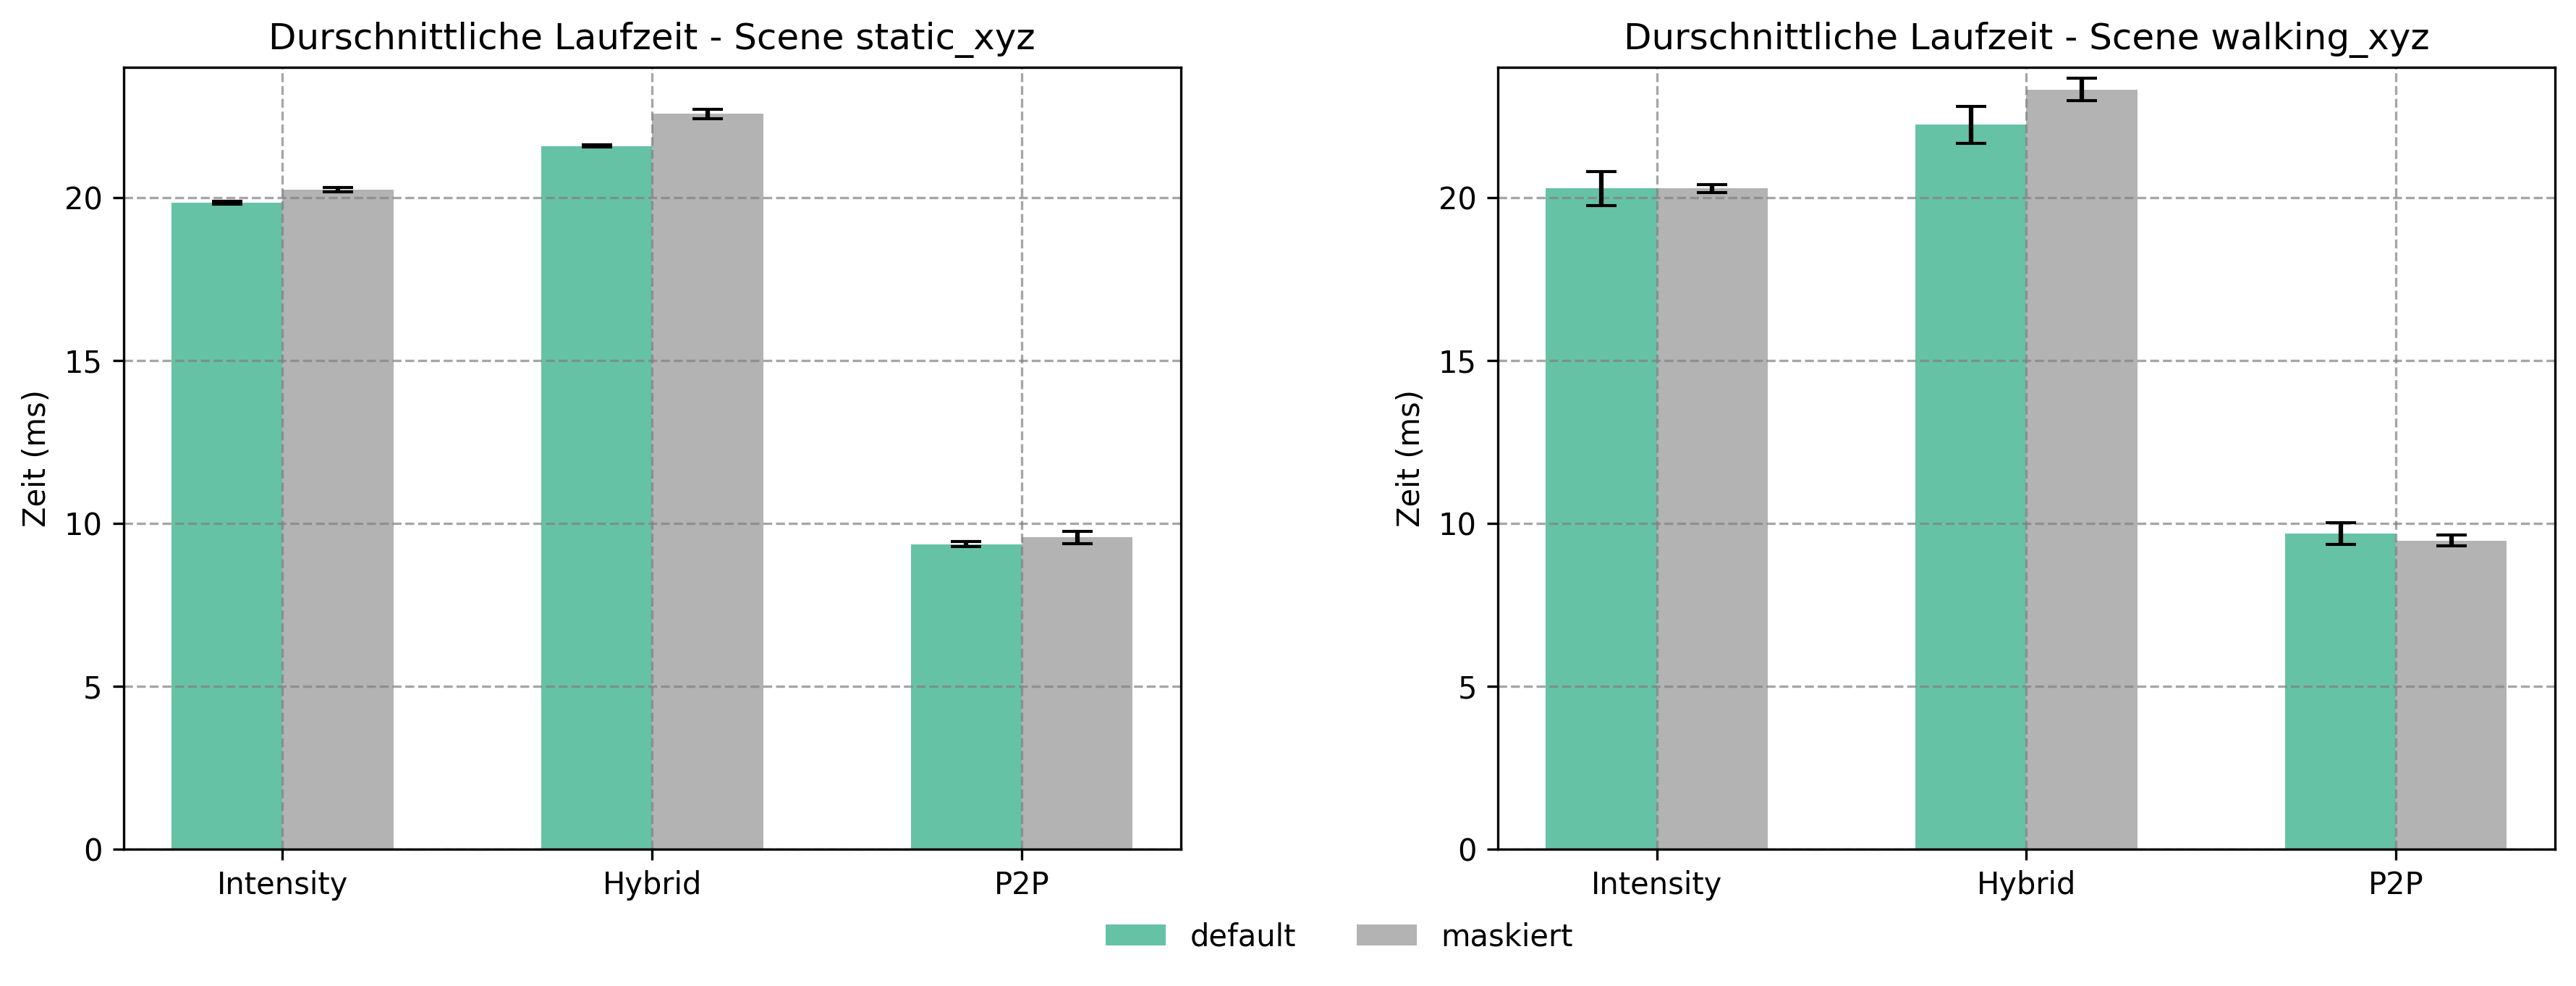
\includegraphics[width=\textwidth]{pics/odom_time_avg.png}
        \caption{durchschnittliche Laufzeit  visueller Odometrie. Vergleich von statischer und dynamischer Umgebung}
        \label{fig:avg_Laufzeit}
    \end{figure} \noindent
    Aus der Grafik \ref{fig:avg_Laufzeit} lässt sich schließen, dass jede Variante des Algorithmus es möglich ist schneller, als die für das dichte Tracking
    übliche Bildrate von 30 FPS, zu laufen. 
    Dabei ist die Laufzeit der Intensität's und Hybrid Fehlerfunktion deutlich höher als die des \ac{P2P}. Dies kann durch eine erhöhte Speicher und 
    Speicherbandbreiten erklärt werden. Auch ist der Rechenaufwand zum Bestimmen der Gradientenbildern über die Sobel-Filter pro Pyramiden-Stufe, ein Faktor.\\\\
    Der Unterschied zwischen der maskierten Variante und der Open3D Implementation ist dagegen kleiner. Das kann mit dem kleineren Speicheraufwand der Masken 
    erklärt werden. Diese werden als 1-Byte pro Pixel Buffer abgespeichert.\\\\
    In statischen Szenen ist die Laufzeit der maskierten Variante geringfügig größer. Jedoch führt die Verringerung der Jacobimatrix Berechnungen 
    bei dem \ac{P2P} in dynamischen Szenen zu einem Laufzeit Ausgleich. Die deutliche Speicher Beanspruchung führt für den Intensity und Hybrid-Fehler
    zu keinen großen Veränderungen.
    \begin{remark}
    In der Laufzeit ist ein nichtlinearer Anstieg im Vergleich zu Speicherverbrauch zu erkennen zwischen 
    \ac{P2P} und den anderen Fehlern. Dies kann mit verbesserten Caching versucht werden zu erklären, da weniger Daten aus
    verschiedene Datenbuffer pro Kernel benötigt werden.
    \end{remark}
    
    \subsubsection{Drift Analyse}
    Visuelle Odometrie bildet einen zentralen Baustein zur Bewegungsbestimmung aus Bilddaten, ist jedoch nicht direkt mit einem \ac{SLAM}-System vergleichbar. 
    Dies zeigt sich auch in Tabelle~\ref{tab:ATE_odom_eval}: Eine durchschnittliche Abweichung von rund einem halben Meter ist für eine präzise Rekonstruktion 
    ungeeignet. Für die Bewertung eines solchen Algorithmus ist daher der \ac{RPE} angebracht.\\\\
    In den Daten \ref{tab:RPE_odom_eval} ist ein klarer Trend erkennbar: Beim Translationsfehler weist das \ac{P2P}-Verfahren einen geringeren Drift auf, unabhängig davon, 
    ob der Bewegung eine Translation oder Rotation zugrunde liegt.\\\\
    Für den Rotationsdrift zeigt sich ein ähnliches Muster, allerdings weniger ausgeprägt, sodass dies nicht zwingend als Beleg für eine höhere rotatorische 
    Robustheit des \ac{P2P} gewertet werden kann.
    Dagegen sprechen insbesondere Szenen mit starker Rotation und ohne dynamische Objekte („static rpy“), in denen das \ac{P2P}-Verfahren deutlich schlechter 
    abschneidet.\\\\
    \begin{figure}[ht]
        \centering
        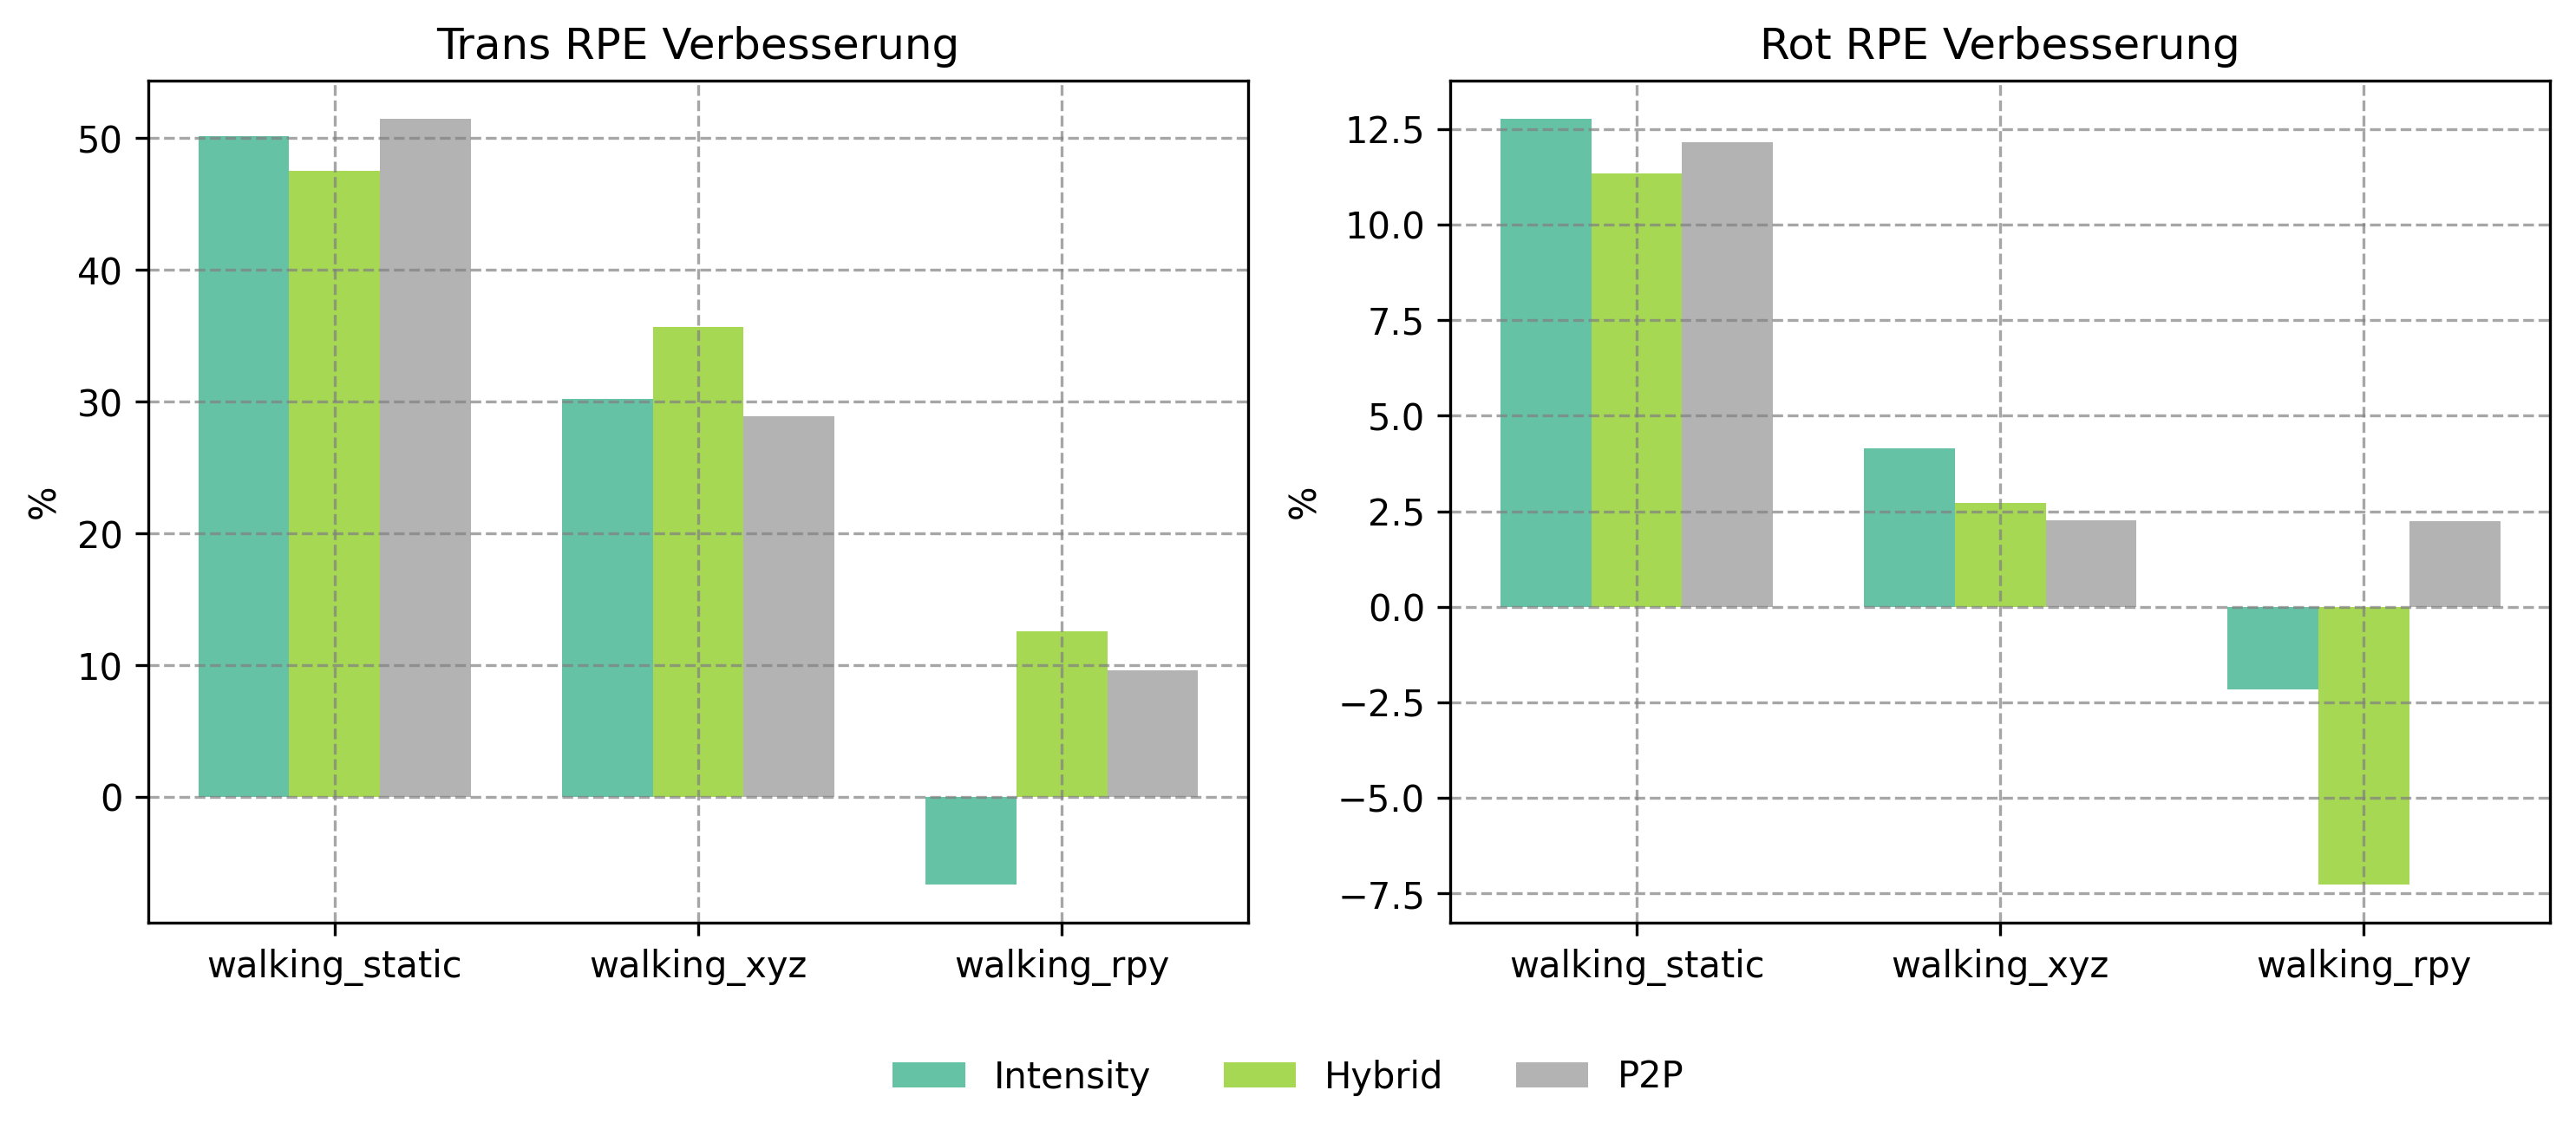
\includegraphics[width=\textwidth]{pics/rel_imp_walking_rpy.png}
        \caption{Prozentuale Verbesserung des RPE durch maskierten Odometrie}
        \label{fig:rel_imp_odom_RPE}
    \end{figure}   
    Auf den statischen Szenen verhalten sich die maskierten Methode gleich zu den unmaskierten. Dies liegt daran, dass die Iteration ohne 
    heraus maskierte Pixel zu den unmaskierten degenerieren.\\\\
    In den dynamischen Szenen zeigt sich eine deutliche Verbesserung des \ac{RPE} (siehe Abb.~\ref{fig:rel_imp_odom_RPE}). Eine Ausnahme bilden die Rotationsszenen: 
    Hier weist ausschließlich das \ac{P2P}-Verfahren eine Verbesserung auf. \\\\
    Aus den dynamischen Szenen mit unbewegter Kamera lässt sich ableiten, dass das Maskieren zu einer stabileren Variante des Algorithmus führt.
    Unter dieser Annahme könnte das Verhalten in den Rotationsszenen als ein generelles Problem der visuellen Odometrie bei starker Rotation interpretiert werden.
    Unterstützt wird diese Annahme durch den in diesen Szenen erhöhten translationalen Drift.
    
    \subsection{TSDF-Tracking Auswertung}
    Der Testaufbau für das \ac{TSDF}-Tracking ist ähnlich zu dem der visuellen Odometrie.
    Dabei wird für die in dem Algorithmus \ref{alg:tsdf_track} genutzte visuelle Odometrie sie selbe Konfiguration genutzt. Das Raycasting Verfahren ist 
    dabei das Standart-Verfahren aus \cite{dong2023ashmodernframeworkparallel}. Die Vergleichs-Version des \ac{TSDF}-Tracking in Open3D nutzt zudem auch ein
    Gewichtungswert pro Voxel um die Stabilität zu erhöhen. Auch in diesem Aufbau wird das Tracking mehrfach auf der gleichen Szene simuliert.
    
    \subsubsection{Laufzeit}
    \begin{figure}[h]
        \centering
        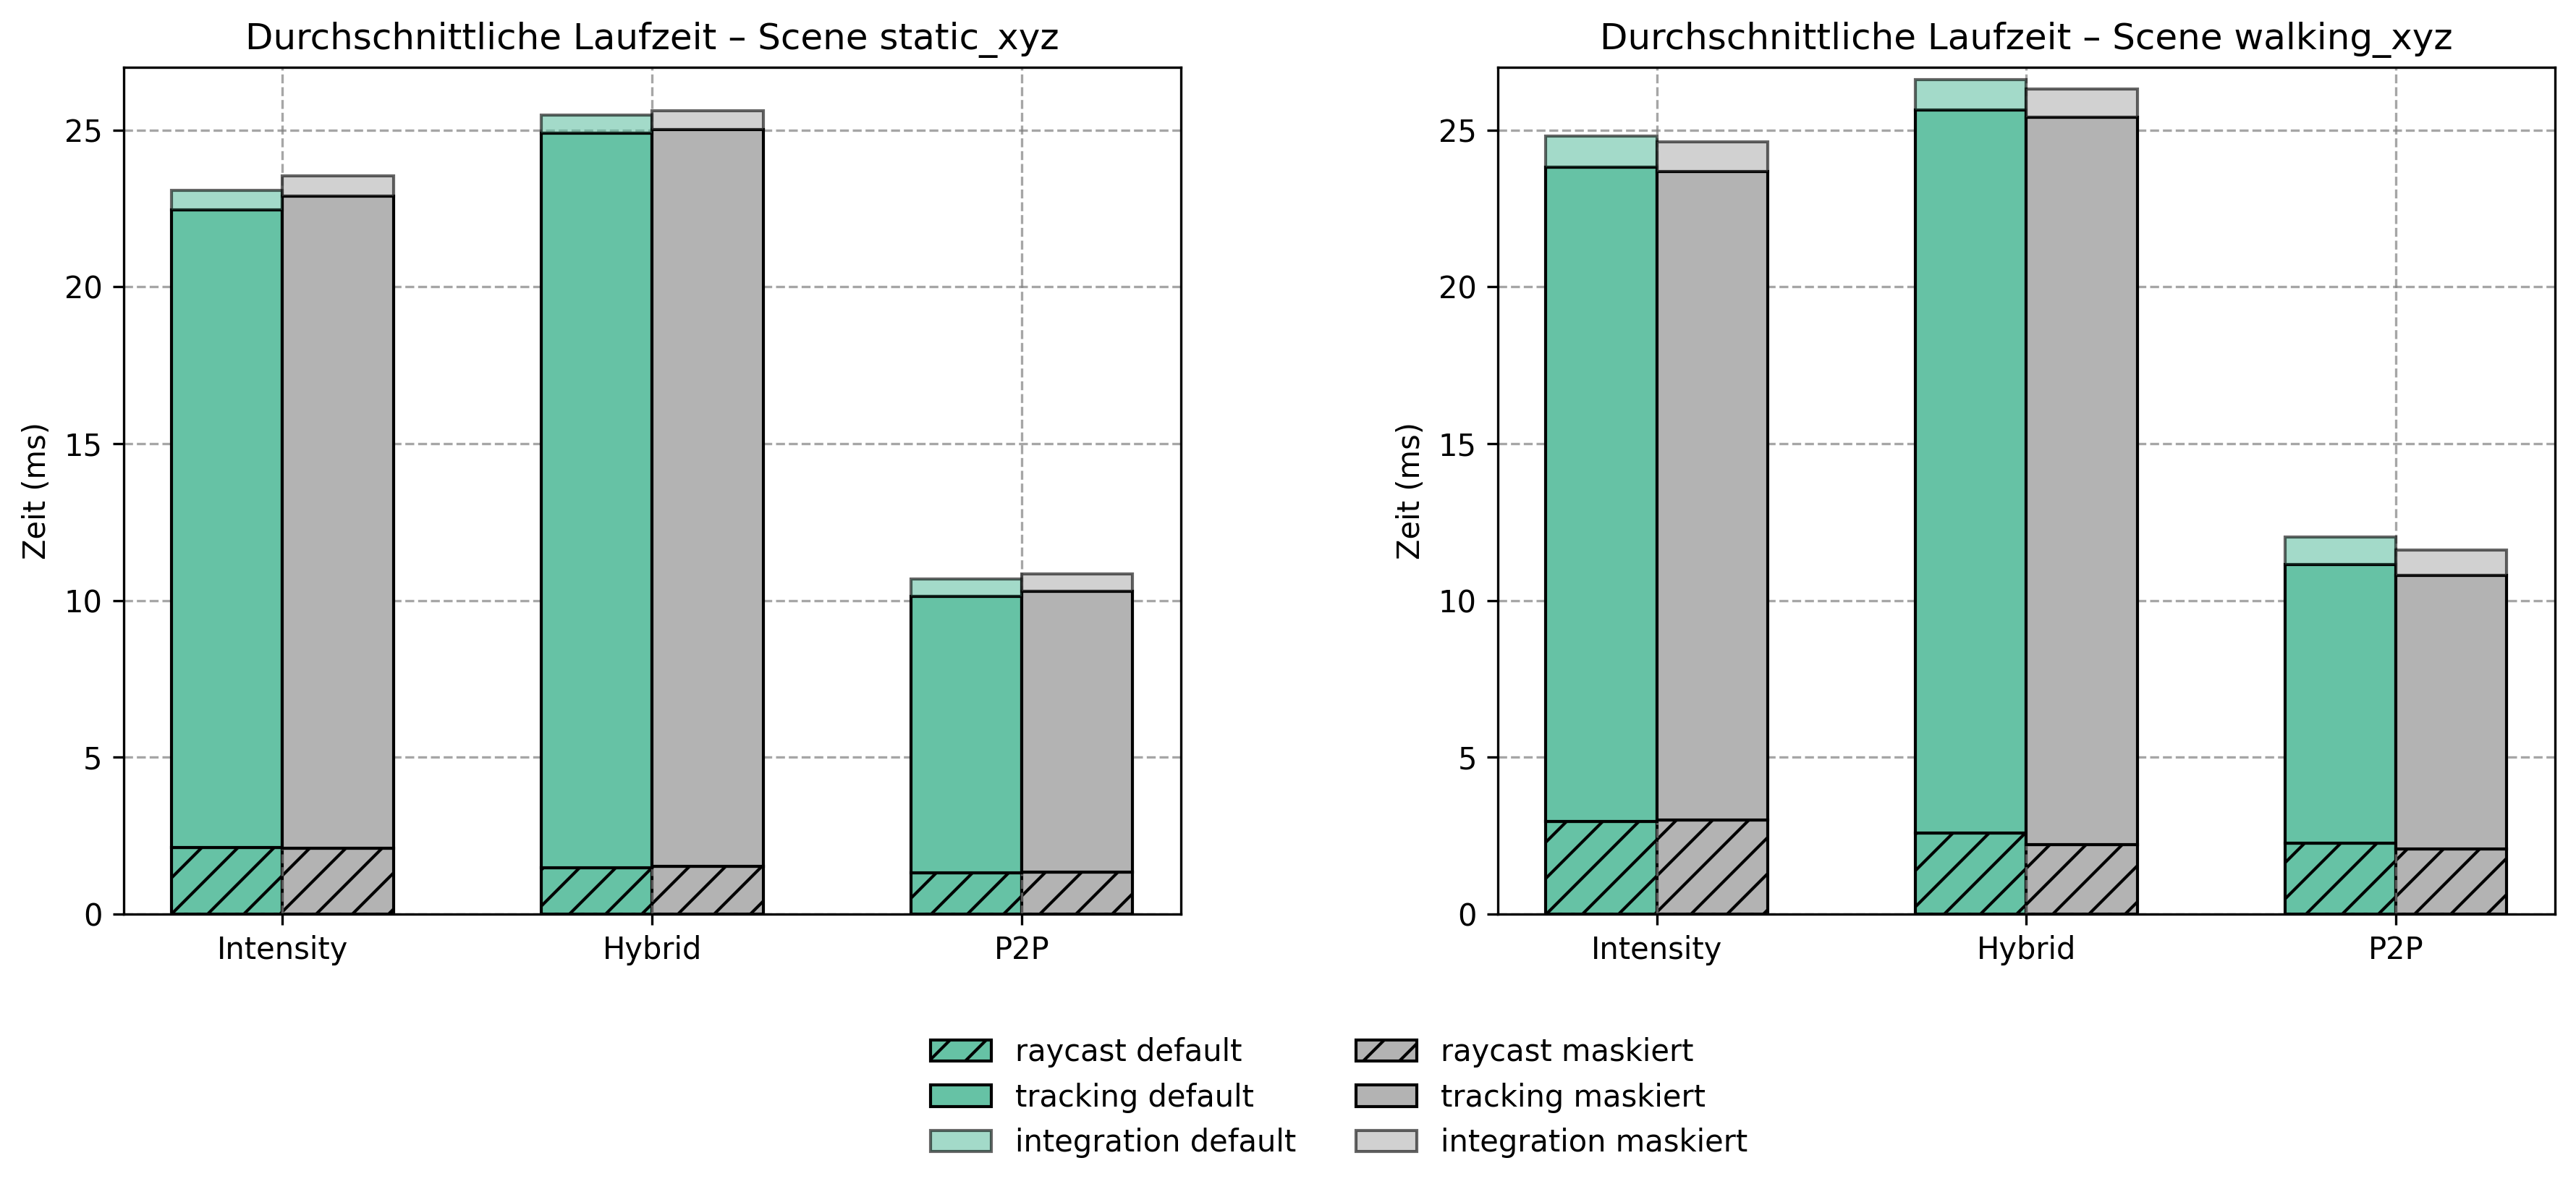
\includegraphics[width=\textwidth]{pics/tsdf_time_avg_split.png}
        \caption{Durchschnittliche Laufzeit des \ac{TSDF}-Trackings}
        \label{fig:tsdf_avg_time}
    \end{figure}\noindent
    Ein Großteil der Laufzeit pro Iteration wird von dem Tracking in Anspruch genommen (vgl. Abb. \ref{fig:tsdf_avg_time}). Dementsprechend ist die das 
    Verhältnis der Laufzeiten fur die verschiedenen Fehlerfunktionen vergleichbar zu Abb. \ref{fig:avg_Laufzeit}. \\\\
    Ein weiteres bobachtes Phänomen ist: Die durchschnittliche Raycasting und Integration Zeit unterscheidet sich zwischen statischer und dynamischer
    Szene. Ein Grund für das Verhalten kann durch die erhöhte Anzahl von aktivierten Blocks und Voxel gefunden werden. In den dynamischen Szenen entsteht
    mehr fehlerhafte Geometrie, die einen negativen Einfluss auf die Rechenzeit des Raycasting under Integration haben. \\\\
    Auch jeder \ac{TSDF}-Algorithmus Variante ist das Echtzeit-Tracking mit einer Bildrate von 30 FPS möglich (auf dem GPU). 

    \subsubsection{Tracking-Verlust}
    Wenn die Daten in den Tabllen \ref{tab:RPE_odom_eval} und \ref{tab:RPE_tsdf_eval} betrachtet werden, fällt auf: Es bestehen starke Schwankungen 
    in \ac{ATE} und \ac{RPE} selbst auf den statischen Szenen. Besonders in den ATE-Werten \ref{tab:ATE_tsdf_eval} sind großen Schwankungen auf der gleichen Szene
    zu beobachten.\\\\
    Dies ist auf ein generelles Problem des Trackings mit einem \ac{TSDF}-VoxelBlockGrid zurückzuführen, dem Tracking-Verlust. 
    Der Voxel Weighting-Mechanismus, der für die Konsistenz des Modells zuständig ist, kann zu einem Verlust der Referenz von Kamera zu Modell führen.
    Durch schnelle Bewegungen kann es passieren, dass Kamerasichtfeld auf noch invalide Geometrie gerichtet ist. Dadurch entstehen unvollständige 
    synthetische Bilder. Das Tracking auf Bildern mit nur wenig validen Pixel kann zu starken Drift, sowie singulären Gleichungssystemen in der visuellen 
    Odometrie führen.\\\\
    Das Verlieren der Referenz für dazu, dass die Kameraposition beliebig driftet bis es wieder ein Modell erstellt wird auf dem getrackt werden kann. Das Ergebnis
    der Rekonstruktion ist dabei Menge von getrackten Fragmenten in unterschiedlichen Orientierung und Abständen.\\\\
    Ein Kriterium um einen Tracking-Loss direkt aus den Daten abzulesen, ist eine hohe Varianz in dem \ac{ATE}. Durch das nahezu zufällige Driften entstehen stark
    unterschiedliche Trajektorien.
    \subsubsection{Fehlerfunktionen}
    Wenn die \ac{RPE} und \ac{ATE} Werte auf den statischen Sznen verglichen werden, ist deutlich zu erkennen, das der \ac{P2P}-Fehler sich am stabilsten verhält. 
    Dies ist gut an der Varianz des \ac{ATE} zu erkennen. Der Intensität's-Fehler ist stark anfällig fur einen Tracking-Verlust (auf jeder Szene). 
    Dies ist auch zu erwarten. Die synthetisch erstellten Bilder simulieren nicht mit akkurate Licht- und Schatten und somit ist ein Vergleich von diesen
    nicht sinnvoll.\cite{dong2023ashmodernframeworkparallel}\\\\
    Ähnliche Probleme sind auch in der Hybrid-Methode zu erkennen. Durch das Einbeziehen der Tiefendaten wird das Tracking verbessert, jedoch tritt auch in 
    der Basis Szenen \glqq static rpy\grqq ein Tracking-Loss auf. Beide Fehlerfunktionen sind nicht für das \ac{TSDF}-Tracking geeignet.\\\\
    Die Fehlerfunktion, die von dem Model profitiert ist die \ac{P2P}. Aus der Abb. \ref{fig:p2p_rel_RPE} ist eine deutlicher Verbesserung des 
    Drifts zu erkennen. Im folgenden wird für das Tracking nur noch der \ac{P2P} betrachtet.
    \begin{figure}[h]
        \centering
        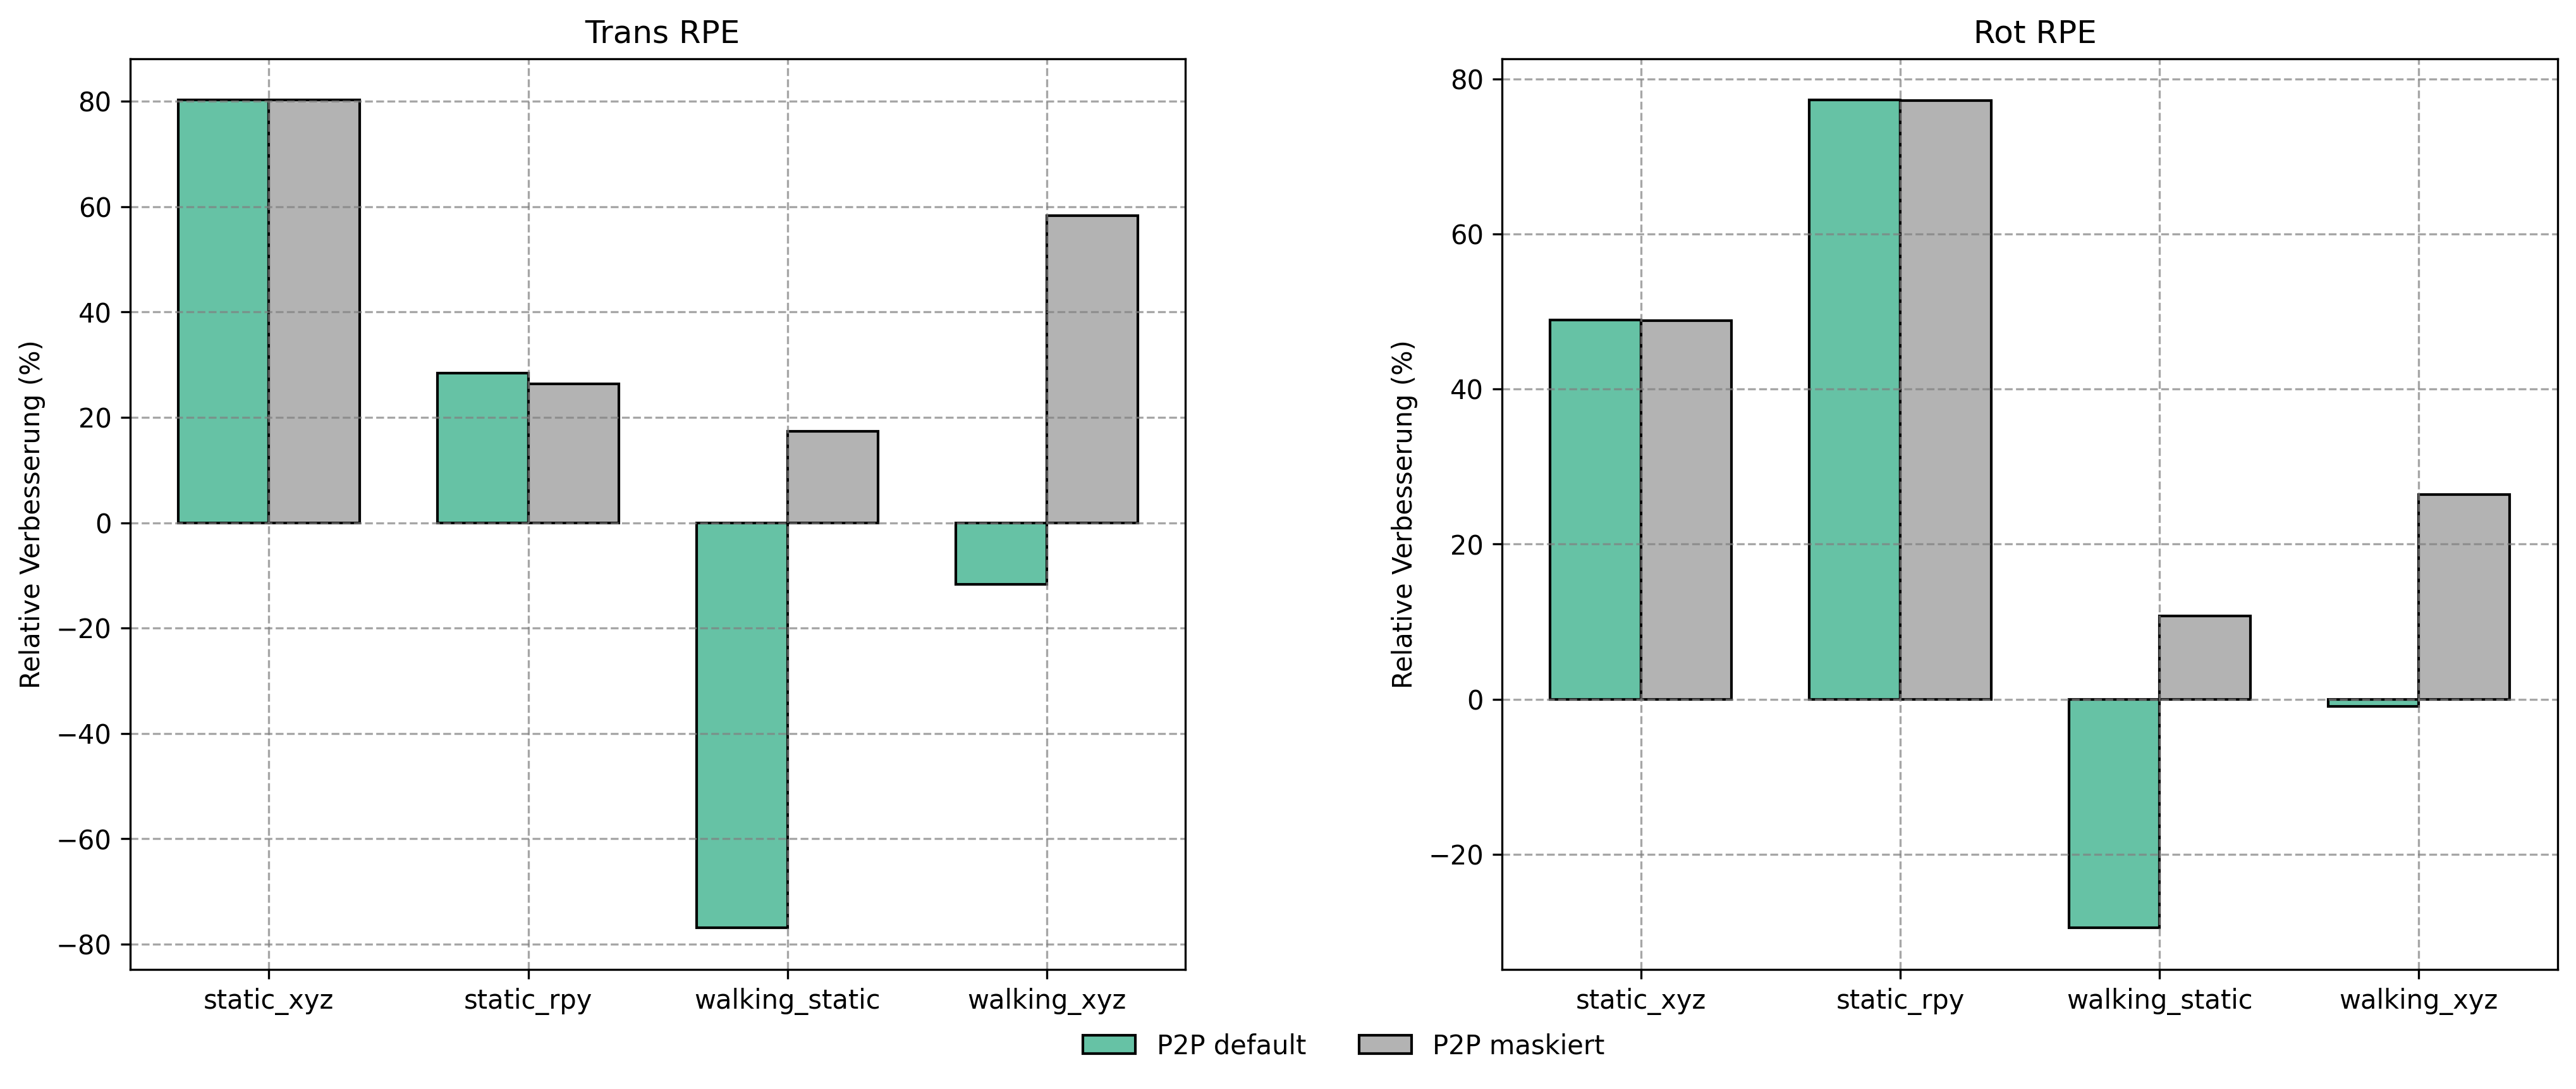
\includegraphics[width=\textwidth]{pics/compose_RPE_com.png}
        \caption{Relative Verbesserung des Drifts der P2P-Fehlerfunktion}
        \label{fig:p2p_rel_RPE}
    \end{figure}

    \subsubsection{Dynamische Szenen}
    In dynamischen Szenen kommt ein weiterer Faktor dazu, der zu einem Tracking-Verlust führen kann. Die Qualität des Trackings hängt stark von der der 
    geraycasteten-Bilder ab. Wenn das \glqq Standard\grqq \ac{TSDF}-Tracking auf den dynamischen Szenen angewendet wird führt dies zu einer Verschlechterung des 
    interne Modell an dem sich das System orientiert (vgl. Abb. \ref{fig:bilder_nebeneinander}).\\\\
    Aus den Varianzwerten des \ac{ATE} auf den dynamischen Szenen ist erkenntlich, dass das \glqq Standard\grqq \ac{TSDF}-Tracking auf jeder das Tracking 
    verliert. Am besten ist dies auf der Szene
    \glqq walking static\grqq zu erkennen. Trotz keiner Kamera Bewegung entsteht ein Tracking-Verlust. Im der Abb. \ref{fig:bild2} ist eine Verschiebung der Szene
    deutlich zu erkennen. \\\\
    \begin{figure}[ht]
        \centering
        \begin{subfigure}[t]{0.45\textwidth}
            \centering
            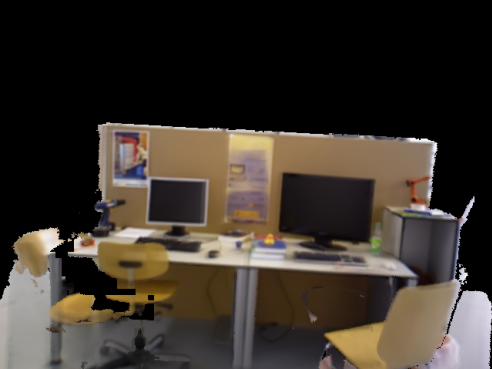
\includegraphics[width=\textwidth]{pics/maskout_image.png}
            \caption{Raycast-Frame maskierte Integration}
            \label{fig:bild1}
        \end{subfigure}
        \hfill
        \begin{subfigure}[t]{0.45\textwidth}
            \centering
            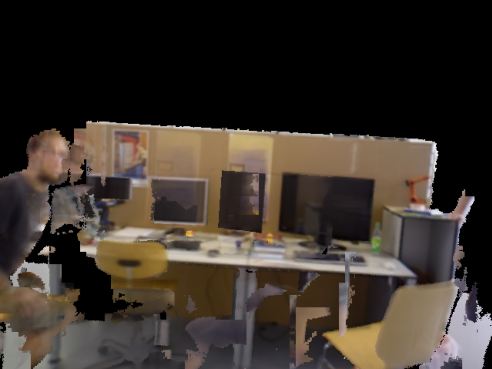
\includegraphics[width=\textwidth]{pics/raw_image.png}
            \caption{Raycast-Frame Open3d standart Integration}
            \label{fig:bild2}
        \end{subfigure}
        \begin{subfigure}[t]{0.45\textwidth}
            \centering
            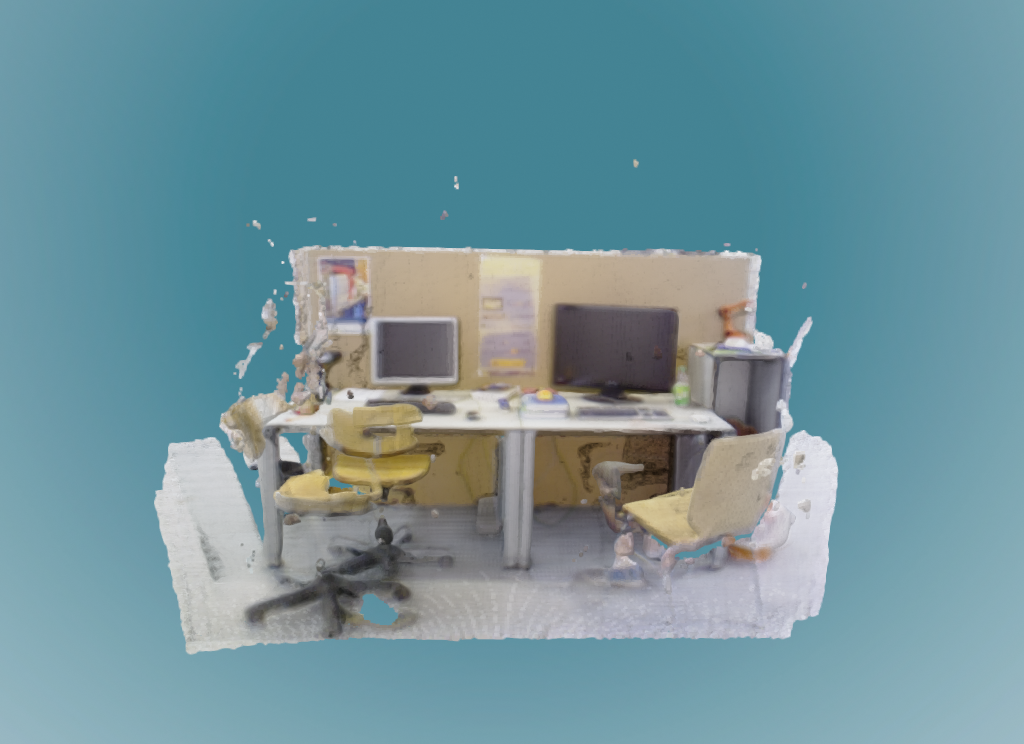
\includegraphics[width=\textwidth]{pics/maskout.png}
            \caption{internes Modell erstellt durch maskierte Integration}
            \label{fig:recon_mask}
        \end{subfigure}
        \hfill
        \begin{subfigure}[t]{0.45\textwidth}
            \centering
            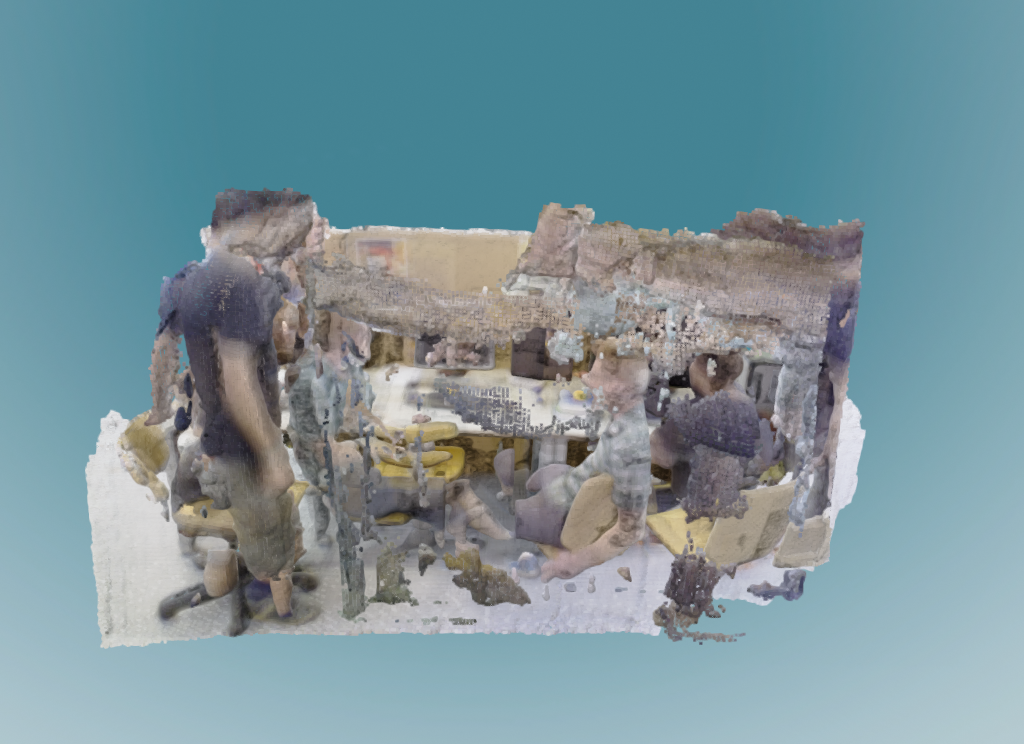
\includegraphics[width=\textwidth]{pics/raw.png}
            \caption{internes Modell erstellt durch Open3d standart Integration}
            \label{fig:recon_raw}
        \end{subfigure}
        \caption{Integrations Algorithmen Vergleich}
        \label{fig:bilder_nebeneinander}
    \end{figure}
    Die maskierte Variante des \ac{P2P} Trackings gelingt es selbst auf den dynamischen Szene eine Tracking-Loss zu vermeiden. Dabei steht die dynamische 
    Roationsbewegungen-Szene hervor. Die Verbindung aus rotation und bewegter Szene erschwert das Tracken immens. Wie schon in Section \ref{sec:aus_vis_odom}
    betrachtet hat der visuelle Odometrie Algorithmus Schwierigkeiten auf der Rotations-Szene.

    \subsection{Bewertung}
    Die beschrieben Experimente zeigen deutlich das der \ac{P2P} den Intensität's und Hybrid Fehler überlegen ist. Das ist leicht in der visuelle Odometrie
    zu erkennen. Inder Laufzeit ist die Fehlerfunktion auch deutlich überlegen. 
    Das Muster setzt sich auch aud das \ac{TSDF}-Tracking fort. Die Trend ist jedoch erwartbar, da die synthetischen Bilder das Tracking per Graustufen behindert.\\\\
    Die  maskierten  Varianten der Methoden stellen eine deutliche Verbesserung in den einzelnen Algorithmen da. Besonders ist dieser Trend bei dem \ac{TSDF}-Tracking
    zu erkennen. Es ermöglicht erst eine Fortsetzung des Verfahrens.\\\\
    Die Ergebnisse zeigen jedoch auch, dass weder die visuelle maskierte Odometrie noch das \ac{TSDF}-Tracking ein zuverlässiges und robustes Tracking gewährleisten.
    Wie in Tabelle~\ref{tab:ATE_odom_eval} ersichtlich, ist die reine Odometrie stark fehleranfällig.
    Das maskierte \ac{TSDF}-Tracking mit der \ac{P2P}-Fehlerfunktion bietet zwar eine deutliche Verbesserung, leidet jedoch unter hoher Instabilität:
    Bei langsamer Bewegung und geringer Rotation arbeitet es zuverlässig, während stark dynamische Bewegungen zu einem vollständigen Trackingausfall führen.\\\\ 
    Somit stellen beide Verfahren für sich genommen kein robustes \ac{SLAM}-System dar.
    Sie können jedoch als Komponenten in einem System eingesetzt werden, das mehrere Tracking-Algorithmen kombiniert und deren Ergebnisse fusioniert.
    Ein solches Zusammenspiel unterschiedlicher Verfahren mit jeweils eigenen Stärken und Schwächen ist charakteristisch für leistungsfähige \ac{SLAM}-Systeme.
    Ein möglicher Ansatz dabei wäre das Tracking durch die visuell basierenden Fehlerfunkionen zu überwachen um einen möglichen Trackingverlust zu erkennen.
    Das führ jedoch in das diverse und umfangreiche Feld der vSLAM-Systeme welche hier nicht betrachtet werden.\\\\
    Für den Einsatz im Stahlumfeld ist das \ac{TSDF}-Tracking trotz der genannten Einschränkungen geeignet. Der Roboter auf dem das System montiert ist bewegt 
    sich mit einer Transitiven Bewegung. Auch ist die Geschwindigkeit des des Roboters gering. In diesem stellt es eine gute Methode da. 

    \chapter{Semantische Bild Segmentierung}\label{sec:SemSeg}

    In dem Gebiet des \ac{vSLAM} sind Deep Learning Methoden essenziell für das Tracking in dynamischen Umgebungen. Dabei sind Bild-Segmentierungs Netzwerke ein 
    wichtiger Bestandteil.\\\\
    Bei der Bildsegmentierung wird unterschieden zwischen der \ac{GIS} und \ac{PIS}. Das automatische Generieren von Masken dynamischer Objekten fällt ind das 
    Gebiet des \ac{GIS} (vgl. \cite{zhou2024imagesegmentationfoundationmodel}). 
    Grundlegende Problemstellungen sind dabei:
    \begin{itemize}
        \item \textbf{Semantische Segmentierung:} Jeder Pixel in einem Bild wird ein Klassenlabel zugeteilt
        \item \textbf{Instanzen Segmentierung:} Pixel werden in zusammenhängende Regionen gruppiert
        \item \textbf{Panoptic Segmentation:} Verbindung Instanzen und semantischer Segmentierung
    \end{itemize}
    Bei der Rekonstruktion der Futterstelle ist es nicht erforderlich zwischen den Kühen zu unterscheiden, deshalb wird hier die Semantischen 
    Segmentierung betrachtet.

    \section{Datensatz}
    Der Datensatz ist eine Menge an Kamerafahrten, die mit an einem Tag in einem Stall aufgenommen wurden. Dabei wird in jeder Kamerafahrt eine Lauf des 
    Schieberoboters simuliert. Sie unterschieden sich untereinander in der Orientierung des Sensors zu der Futterstelle.\\\\
    Die Bilder stellen hoch dynamische Szenen da, mit vielen sich im Hintergrund und Vordergrund bewegenden Kühen. Viele Kühe sind dabei Großteil verdeckt oder 
    klein in dem Hintergrund. Auch herrschen teilweise schlechte Lichtverhältnisse, die die Qualität der Bilder mindert.
    Insgesamt besteht der Datensatz aus 6 Läufen und insgesamt 350 Bildern. Die Auflösung der Bilder in dem Datensatz ist 640x480.\\\\ 
    Die in dem Datensatz annotierten Klassen sind:
    \begin{itemize}
        \item \textbf{Kühe:} Für das Maskieren in den Tracking und Rekonstruktion-Algorithmen
        \item \textbf{Silage:} Als Grundlage in der Futtermessung
        \item \textbf{Background:} Die restliche Szene
    \end{itemize}\noindent
    Durch die Unterschiede der Kamera-Positionierung herrscht in bestimmten Kamerafahrten eine starke Klassen-Ungleichheit. Dabei stellt der Hintergrund und die Silage
    einen Großteil der Pixel da. In anderen Kamerafahrten dominieren die Kühe als Klasse die Bilder.

    \subsection{Annotation}
    Die Annotation stellt einen aufwendigen Teil in der Erstellung des Datensatzes da. Für die semantische Segmentierung muss eine Klassifikation pro Pixel annotiert 
    werden. Aufgrund des hohen Aufwandes werden schon existierende Segmentierung in den Labeling Prozess mit eingebunden.\\\\
    Die einfache Nutzung von \ac{GIS} Segmentierungsmodell führt zu Schwierigkeiten. Aufgrund der Komplexität der gefilmten Szene,
    sowohl als auch der spezifischen Anforderungen der Klassen, ist viel manuelles Postprocessing nötig.\\\\
    Für effektiveres Labeln können \ac{PIS} Segmentierungs-Modells genutzt werden. Konkret wurde das SAM2 \cite{ravi2024sam2segmentimages} verwendet. Das Modell 
    bietet die Möglichkeit Segmentierung aufgrund von Promts zu erreichen. Dafür können Punkte, Bounding-Boxes und Vorsegmentierung als Input in das Modell gegeben 
    werden um Regionen zu spezifizieren. Dies erlaubt ein flexibles und schnelles Segmentieren von selbst schwer semantisch zu erkennenden Regionen.\\\\
    Selbst mit dem flexiblen Labeling Setup ist noch manuelles Postprocessing nötig, für schwer zu erkennende Regionen.
    Die Segmentierungen sind nicht pixelgenau. Aufgrund ungünstiger Lichtverhältnisse lassen sich Kühe im Hintergrund teilweise nur schwer oder gar nicht erkennen.

    \subsection{Evaluation und Trainingsdatensatz}
    Der Datensatz weist einige Herausforderungen auf. Bilder aus demselben Durchlauf sind aufgrund temporaler Überschneidungen stark miteinander korreliert.
    Daher ist bei der Trennung in Trainings- und Evaluationsdaten besondere Vorsicht geboten.
    Ein akkurates Vorgehen wäre, Trainings- und Evaluationsdatensatz aus Aufnahme aus verschiedenen Ställen zu verwenden. Das ist jedoch zu diesem
    Zeitpunkt nicht möglich, da bislang nur an einem Tag in einem einzigen Stall aufgezeichnet wurde. Zukünftig ist geplant, den Datensatz in dieser Hinsicht 
    zu diversifizieren.\\\\
    Auf dem momentanen Datensatz ist ein sauberes Vorgehen eine direkte Trennung der Kamerafahrten. 
    Das dabei erstehende Problem ist, dass eine Imbalance zwischen der Anzahl der Bilder in den einzelnen Läufen besteht.
    Das führt dazu, dass eine faire Trennung nicht ohne große Variation der große des Evaluationsdatensatz oder einem Verlust von annotierten Bilder möglich ist.\\\\
    Die deshalb gewählte Trennung besteht aus einer Unterteilung in den Kamerafahrten. Damit die Trainings und
    Evaluationsdatensatz nicht zu stark korrelieren werden zeitliche Pufferzonen eingebaut. Diese Lösung ist nicht optimal, da trotzdem starke Zusammenhänge 
    zwischen Splits bestehen.
    
    \subsection{Crossvalidation}
    Die Wahl der Splits beinflusst stark zeitliche Position der Evaluation's-Bilder. Um diesen Faktor zu gut wie möglich zu kontrollieren wird
    ein Teilung mithilfe von 5-Folds Crossvalidation festgelegt. Dabei werden die temporalen Abschnitte zufällig in jeder Fahrt gewählt, ohne das dabei
    einen eine Menge von Bildern mehrfach als Validationsdatensatz vorkommt.\\\\
    Der Testdatensatz stellt eine extra annotierte Fahrt da, die nicht in die Crossvalidation eingeht. Jedoch stammt er von dem selben Tag und Stall, was die 
    Genrealisierbarkeit, der auf ihm erzielten Ergebnisse deutlich infrage stellt.

    \subsection{Augmentation}
    Aufgrund der kleinen Große des Datensatzes werden die Bilder im Training konstant augmentiert. Dafür wird eine zufälliger Spiegelung und eine zufälliger
    Verkleinerung um 20 \% des Bildbereiches auf ein Bild angewendet (vlg. \cite{chen2017rethinkingatrousconvolutionsemantic,HaitzHuebnerUlrich2022}).  
    Auch wird die Helligkeit und der Kontrast zufällig variiert. Dies soll die schwankende Lichtverhältnisse im Stall emulieren.

    \section{Architektur}
    Eine klassische Herangehensweise semantische Segmentierung zu erreichen ist es, bewehrte Modelle aus der Bildklassifikation zu modifizieren.\\\\
    Die hier genutzte Architektur ist die DeeplabV3plus. Dabei stellt ein \ac{CNN} die Grundlage
    bzw. den sogenannten Backbone da. Die Idee ist, dass das Backbone Netzwerke die sogenannte Feature Extraction (das effiziente erkennen von
    hochdimensionen Bildstrukturen) effizient durchführt, aufgrund welcher die Pixel klassifizierte werden.
    \cite{chen2018encoderdecoderatrousseparableconvolution}

    \subsection{CNN}
    Für diese Idee muss zuerst die Architektur und Funktionsweise von CNN's verstanden werden. Die grundlegende Operation, die CNN's ihren Namen gibt, 
    ist die Convolution (Faltung). Diese stellt eine Möglichkeit da, lokal Bild Information zu erfassen.
    \begin{defi}
    Sei $\Omega := \{0, \ldots , W-1\} \times \{ 0, \ldots, H-1\} \times  \{ 0, \ldots,C_{in}\}$, dann wird ein Bild (Feature Map), mit Auflösung $H\times W$ 
    und $C_{in}$ Featurechannels, definiert durch $I: \Omega \to \mathbb{R}$.\\\\
    Weiter sei $\Omega^* := \{0, \ldots , k_w\} \times \{ 0, \ldots, k_h\} \times \{0, \ldots, C_{in} \} \times  \{0, \ldots,C_{out}\} $. Dann ist ein 
    Convolution Kernel (Faltungskerne) mit Kernel Größe $k_w  \times k_h$ für $C_{in}$ Input Feature Channels Feature Channels und $C_{out}$ Output 
    Channels gegeben durch $K: \Omega^* \to \mathbb{R}$.\\\\
    Eine $k_w\times k_h$ Bildfaltung (Image-Convolution) zu dem Kernel K, ist definiert als:  
    \[
    (I * K)(x, y, c) = \sum_{i =0}^{k_h-1}\sum_{j=0}^{k_w-1} \sum_{d = 0}^{C_{in}-1}I(x-i +a, y-j+b, d)K(i,j,d,c)
    \]
    Dabei sind $a = \lfloor \frac{k_w}{2} \rfloor, b = \lfloor \frac{k_h}{2} \rfloor$. Eine Convolution mit $K$ erzeugt ein neues Bild $I * K$ 
    mit $C_{out}$ Feature Channels.\cite{pytorch_Convolution}
    \end{defi} 
    \begin{remark}
    Wenn sich die Definition einer Bildfaltung angeschaut wird fällt auf, dass die Abbildung nicht für alle $(x,y,c)$ definiert ist.
    Dies passiert dadurch, dass für die $(x,y)$ am Rand des Bildes $(x-i+a,y-j+b) \notin  \{0, \ldots , W-1\} \times \{ 0, \ldots, H-1\}$.
    Effektiv verkleinert sich also die Auflösung des Output Bildes $I * K$. Dies wird in der Praxis durch Padding, das Erweitern des 
    Definitionsbereiches des Input Bildes durch Default Werte, gelöst. \cite{pytorch_Convolution}    
    \end{remark}\noindent
    Die Faltung mit einem Kern $K$ stellt eine gewichtet Summe über die Feature Channel einer lokalen Umgebung $k_w, k_h$ da. Dies passiert
    für jeden Output Feature Channel. Damit soll es den Modellen ermöglicht werden unterschiedliche Aspekte des Bildes zu extrahieren.\\\\
    Ziel ist es die Anzahl der Output Channels  eines neuen Bildes zu erhöhen, damit über die Channels ein Klassifikation gemacht 
    werden kann. Dies ist jedoch nicht ohne weiteres möglich da der Speicherplatz linear in den Channel Ansteigt. Deshalb ist die Strategie 
    von CNN's die Auflösung $H\times W$ zu reduzieren und gleichzeitig die Anzahl der Feature Channels zu erhöhen. Hierzu werden sogenannte strided 
    Convolutions genutzt.
    \begin{defi}
    Sei I ein Feature-Map und $K$ ein Faltungskern. Weiter seien $s_h, s_w \in \mathbb{N}$, dann ist die 
    strided Bildfaltung zu dem Kernel K definiert durch 
    \[
    (I * k)(i, j, c) = \sum_{i =0}^{k_h-1}\sum_{j=0}^{k_w-1} \sum_{d = 0}^{C_{in}-1}I(x *s_h-i +a, y*s_w-j+b, d)K_{i,j,d,c}
    \]
    \end{defi}\noindent
    Die Werte $s_h, s_w$ stellen die Schrittweiten der Mittelpunkte des Kernelfenster da. Mit geschickter Wahl von Padding und Schrittweiten wird 
    die Auflösung der Bilder halbiert und gleichzeitig die Anzahl der feature Channels verdoppelt. Der Faktor um den Auflösung reduziert 
    wird, wird als der Outputstride bezeichnet. Viele Modelle haben eine Outputstride von 32 und größer. Auf diesen Feature-Maps mit kleiner Auflösung und vielen 
    Features-Channels wird dann eine Klassifikation durchgeführt.

    \subsection{Encoder}
    Der Encoder von Deeplab besteht zum großen Teil aus dem Backbone Model. Dieses liegt jedoch in modifizierter Form vor.
    Das Problem welches auftritt, wenn das unveränderte Backbone Model genutzt wird ist, dass der Outputstride sehr groß ist. Um also auf die originale Auflösung zurück 
    zukommen muss die Klassifikation dementsprechend hochskaliert werden, was zu einer groben Akkuratheit der Pixel führt. Um das Problem zu umgehen wird versucht den 
    Outputstride so klein wie möglich zuhalten.
    \subsubsection{Atrous Convolutions}
    Dies bringt jedoch Probleme mit sich. Convolutions in späteren Schichten haben die die Eigenschaft, dass sie durch die Verringerung
    der Auflösung größere Bildbereiche wahrnehmen. Um das Verhalten zu emulieren werden sogenannte Atrous Convolutions genutzt. 
    \begin{defi}
    Sei I ein Bild und $K$ ein Faltungskern. Weiter seien $r_h, r_w \in \mathbb{N}$, dann ist die 
    Atrous Bildfaltung zu dem Kernel K definiert durch 
    \[
    (I * k)(i, j, c) = \sum_{i =0}^{k_h-1}\sum_{j=0}^{k_w-1} \sum_{d = 0}^{C_{in}-1}I(x-i*r_h +a, y-j*r_w+b, d)K(i,j,d,c)
    \]
    \end{defi}
    Atrous Convolutions simulieren eine Ausbreitung des Faltungsfensters. Ab einem bestimmten Outputstride werden stridet Convolution durch 
    die entsprechenden Atrous Convolution ersetzt \cite{chen2017rethinkingatrousconvolutionsemantic}.
    \begin{remark}
    \label{bem:backboneparam}
        In der Implementation werden vortrainierte Parameter von dem Backbone Model genutzt werden (vgl. \cite{chen2017rethinkingatrousconvolutionsemantic,HaitzHuebnerUlrich2022}). 
        Da die Anzahl der In- und Output-Channels unverändert bleibt, 
        sowie die Dimension der Kernelfenster, stimmen die Dimension für die Parameter überein. Auch bleibt der Sichtbereich der Fenster durch die 
        Ausbreitung gleich, was eine Rechtfertigung für die Sinnhaftigkeit der Parameter des Backbone-Models gibt.\\\\
        Wichtig dabei ist anzumerken, dass aufgrund der höheren Auflösung der Speicherplatz der Feature Maps ansteigt, sowie der Rechenaufwand, da die Fenster auf 
        mehr Pixel operieren . \cite{Deeplabv3plus_PyTorch}
    \end{remark}

    \subsubsection{Seperable Convolutions}

    \subsubsection{Astrous Spatial Pyramid Pooling}
    Eine weitere Strategie um Features auf unterschiedlichen Skalen zu lernen, ist das \ac{ASPP}. Dabei wird auf die letzte Feature
    Map mehrere separable Atrous Convolution mit unterschiedlichen Raten und Padding in parallel angewendet. Zudem wird noch eine 1x1 Convolution $(k_w = k_h = 1)$
    und ein 2x2 Average Pooling Layer angewendet. Das Padding in den Atrous Convolution wird dabei so gewählt, dass die Auflösung der Feature Map erhalten
    bleibt. Der Output des Pooling Layers wird dabei auf die Auflösung hoch interpoliert. Der Output wird aneinander gehängt und Mithilfe von einer 
    weiteren 1x1 Convolution werden die Feature Channels auf runter projiziert.\cite{chen2017rethinkingatrousconvolutionsemantic}
    
    \begin{figure}[ht]
        \centering
        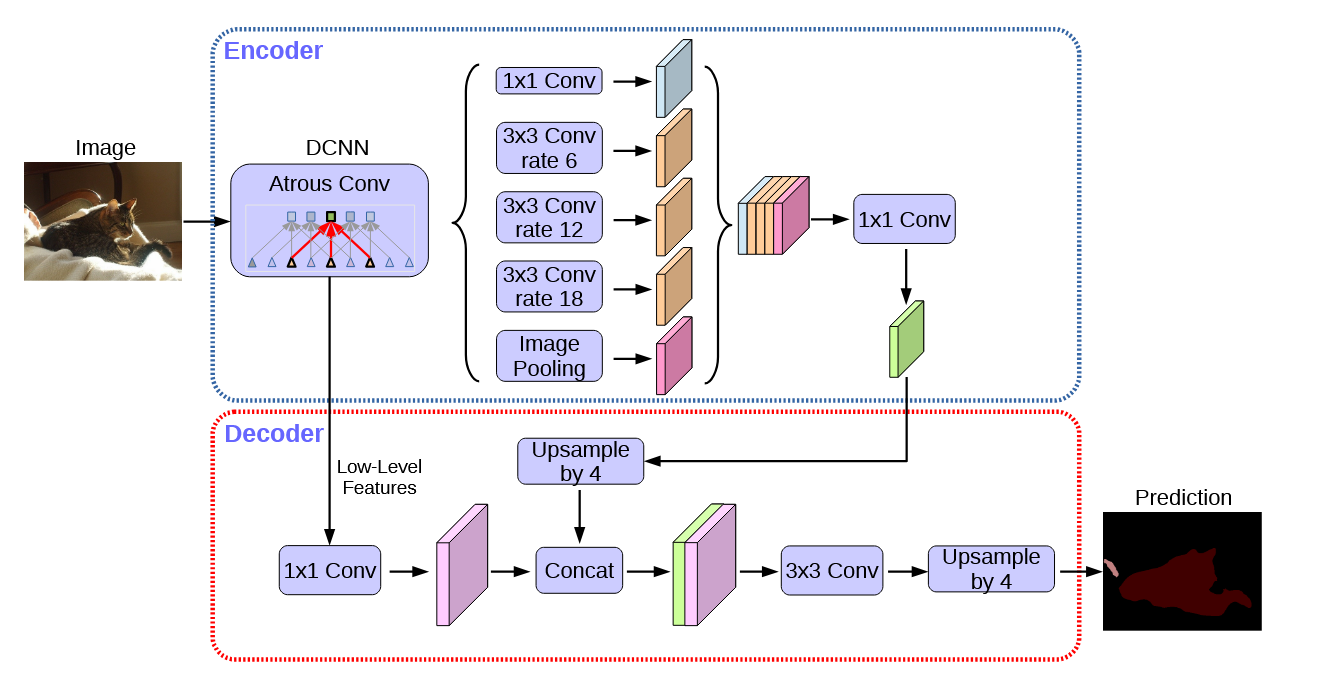
\includegraphics[width=0.9\linewidth]{pics/Arc.png}
        \caption{DeepLabv3+ Architecture (Original aus \cite{chen2018encoderdecoderatrousseparableconvolution})}
        \label{fig:deeplabv3plus}
    \end{figure}

    \subsection{Decoder} 

    Frühere Deeplab Models hatten nur einen primitiven Decoder, der die Ergebnisse des \ac{ASPP} Modules nur Bilinear auf die originale
    Auflösung hoch interpoliert. In den Paper \cite{chen2018encoderdecoderatrousseparableconvolution} wird ein komplexerer Decoder präsentiert, 
    der den Process des Hochskalierens erleichtert.\\\\
    Die Idee ist eine Feature Map aus dem Backbone Model mit höherer Auflösung und groberen Features zu speichern während der Inference 
    und dann diese bei der Hochskalierung zu nutzen. Ziel dabei ist es schärfere lokale Segmentierung zu erreichen. 
    Dafür wird die Faturemap mit einem Outputstride von 4 genommen, die sogenannten Low-Level-Features \cite{chen2018encoderdecoderatrousseparableconvolution}. 
    Das \ac{ASPP} Module bleib wie es ist und wird bei einem Outputstride von 8 oder 16 angewendet \ref{fig:deeplabv3plus}.\\\\
    Die Ergebnisse werden Bilinear hoch interpoliert, bis auf den Outputstride 4. Die Anzahl der Feature-Channels in den Low-Level-Features wird durch
    eine 1x1 Convolution reduziert und darauf hin mit den hochskalierten High-Level-Features aneinander gehängt.\\\\ 
    Eine darauf folgenden 3x3 Convolution, auf den kombinierten Feature soll eine Verfeinerung der High-Level-Features Auflösung durch die 
    Low-Level-Features erreichen. Erst dann wird die finale Klassifikation der Features durch eine 1x1 Convolution erreicht.


    \section{Trainingskonfiguration}
    Für das Training des Model wurde eine modulare Implementation von dem Deeplabv3plus Model in Pytorch gewählt \cite{Deeplabv3plus_PyTorch}. Das Repository erlaubt
    es vortrainierten Parameter einfach für verschiedene Backbone Modelle zu laden. Dabei stehen die Modelle ResNet, MobilenetV2, Xception, und Hrnet zu Verfügung.
    Somit ist es möglich folgenden Experimente mit unterschiedlichen Modell einfach fortzusetzen.\\\\
    Als Backbone-Model für die Experimente wurde das ResNet-50 gewählt. Es handelt sich um ein neuronales Netz, das auf Standard-Convolutions basiert.
    Im Gegensatz dazu setzen Modelle wie MobileNetV2 oder Xception auf Depthwise-Separable-Convolutions, was zu deutlich weniger Parametern und geringerem 
    Rechenaufwand führt. Die ResNet Architektur wird auch als Backbone in dem Paper \cite{chen2017rethinkingatrousconvolutionsemantic,HaitzHuebnerUlrich2022} 
    genutzt und stellt ein bewährtes Modell da.\\\\
    ResNet-50 weist daher eine höhere Parameteranzahl und einen größeren Rechenaufwand auf, bietet aber auch ein höheres Potenzial für 
    maximale Genauigkeit. Die Wahl fiel bewusst auf ResNet-50, um das Leistungspotenzial des Ansatzes zu evaluieren. In späteren Trainingsiterationen ist vorgesehen, 
    auch ressourcenschonendere Backbones zu untersuchen, die sich für effiziente Systeme besser eignen.\\\\
    Das ResNet50 ist eine kleinere Version des ResNet Modells, mit 50 Schichten, was es ermöglicht es auf Verbraucher freundlichen Hardware zu Trainieren. Die 
    vortrainierten Parameter stammen aus dem Torchvision Modul und wurden auf dem ImageNet-1k Datensatz \cite{deng2009imagenet} trainiert.
    Dabei wurden nur die Parameter von einem Datensatz genutzt, da in \cite{HaitzHuebnerUlrich2022} kein starker Einfluss durch den Datensatz auf festgestellt werden
    konnte.

    \subsection{Hyperparameter}
    Die Konfiguration fur Training des Modells bietet eine Vielzahl von zu wählenden Parameter. Diese  Hyperparameter werden nicht durch den Traningsprozess optimiert,
    sondern müssen im Vorhinein gewählt werden.
    \subsubsection{Loss}
    Für die Bildsegmentierung, sowie allgemein Klassifikation-Problemen ist der Cross-Entropy-Loss eine gängige Fehlerfunktion 
    (siehe \cite{chen2017rethinkingatrousconvolutionsemantic}).
    \begin{defi}
    Sei $C \subset \mathbb{N}$ die Menge der Klassen. Weiter $x_i, i \in C$ die Ausgabe des Modells zu der Klasse $i$. 
    Weiter sei $w_i$ eine Gewichtung der Klasse $i$. Der Cross-Entropy-Loss für die Ausgabe $x$ des Modells yu dem Label $y$ ist definiert durch
    \begin{equation}\label{def:cross_entr}
        l_{cross}(x,y) = -w_{y} log\left(\frac{exp(x_{y})}{\sum_{c=1}^{C}exp(x_{c})}\right)
    \end{equation}
    \end{defi}\noindent
    Der Gewichtungswert wird für das manuelle Ausgleichen von Klassenungleichgewichten genutzt. In dem Fall des Datensatzes wird nur die Hintergrund 
    Gewichtung angepasst mit der Range $[0.1,1]$.\\\\
    Ein weiterer Loss, der besonders in der Bild-Segmentierung genutzt wird ist der Focal-Loss.
    \begin{defi}
    Sei die Notation gleicht zu der in \ref{def:cross_entr}. Dann ist der Focal-Loss gegeben durch (vgl.\cite{lin2018focallossdenseobject}). 
    \begin{equation}
        l_{FL}(x,y) = -\alpha (1-p)^{\gamma}log (p)
    \end{equation} 
    \end{defi}\noindent
    Der Focal-Loss stellt eine adaptive Gewichtung des Cross-Entropy-Losses da, bei dem Pixel mit hoher vorhergesagter Confidence geringer und Pixel mit 
    niedriger Confidence hoher gewichtet werden. Der Vorteil ist, dass automatisch der einen Fokus auf schwer zu klassifizierende Pixel gelegt wird. Dabei 
    kann dies bei ungenauer Pixel Annotation zu Trainingsschwierigkeiten führen.
    \subsubsection{Weight-Decay}
    Der Weight-Decay stellt eine Regularisierung des Modells im Training da, um Overfitting zu vermeiden. Dabei wird ein Regularisierungsterm in die Fehlerfunktion
    hinzugefügt, der eine Gewichtung der Norm des Modell-Parameter darstellt.  
    \begin{equation}
        l_{L2}(x,y) = l(x,y) + \lambda ||W||^2
    \end{equation}
    $W$ stellt den Vektor mit allen trainierebaren Parametern des Modells da. $\lambda$ ist der Weight-Decay Faktor gewählt wird. Er stellt die Gewichtung zwischen 
    Fehlerfunktion und Größe des Modell Modells da. Dadurch soll die Komplexität eines Modells betraft werden um Overfitting  auf dem Trainingsdatensatz zu vermeiden.

    \subsubsection{Optimierer}
    Für das Training wurde der AdamW-Optimierer eingesetzt. AdamW ist ein Variantenoptimierer auf Basis von Adam, bei dem das Weight-Decay korrekt vom 
    Gradientenupdate entkoppelt ist \cite{loshchilov2019decoupledweightdecayregularization}. Er stellt einen robusten Optimierer für Tiefe \ac{CNN}'s
    da. Dabei ist im Gegensatz zu oft dem genutzten Momenten basierte Stochastic-Gradient-Decent ein geringe Wahl von Hyperparameter nötig. Hier wird 
    nur die Lernrate optimiert.

    \subsubsection{Backbone Training}
    Aufgrund der Größe des Datensatzes ist es nicht nicht sinnvoll ein Tiefes Convolutionelles Modell zu Trainieren. Um das Problem zu umgehen wird versucht
    die vortrainierte Parameter effektiv zu nutzen. Dazu wird für das Backbone-Modell die Lernrate um einen Faktor von 0.1 verringert. Diese Strategie wird auch
    in den Paper \cite{chen2017rethinkingatrousconvolutionsemantic} genutzt.\\\\
    Eine andere Herangehensweise ist es die Parameter aus dem Training komplett zu entfernen. Dabei muss beachtet werden nur die Parameter zu entfernen die auch
    unverändert auf der jeweiligen Feature-Map operieren. Wenn also eine Erhöhung eine strided Convolution durch eine Atrous-Convolution vertauscht wird, operieren
    die Erweiterten Convolutions auf dem gleiche Sichtfenstern, aber auch auf einer größeren Feature-Map (Bem. \ref{bem:backboneparam}). Aus diesem Grund sollten sie in 
    das Training einbezogen werden.
    \subsubsection{Outputstride}
    Für die Konfiguration des Backbone-Models muss auch der Outputstride festgelegt werden. Dabei stehen 8, 16 praktisch zur Auswahl. Ist der Outputstride zu klein 
    steigt der Rechenaufwand, sowie der Speicherverbrauch dramatisch an \cite{chen2017rethinkingatrousconvolutionsemantic}. Ist er zu klein kann es zu unpräzisen
    Versagen führen, da der Up-Sampeling Faktor zu groß ist, selbst mit Hilfe der hinzugefügten Decoders.

    \subsection{Hyperparameter Optimierer}
    Aufgrund des kleinen Trainingsdatensatzes ist die Konfiguration der Parameter schwer im Vorhinein eingrenzen durch fehlende Referenz Experimente.
    Die Konfiguration Bereiche sind große gewählt um Preconditioning des Trainings zu vermindern. Für die Bestimmung einer guten Konfiguration wird
    eine Kombination aus Exploration und Exploitation genutzt.\\\\
    Für die Hyperparameter-Optimierung wird eine Kombination aus einem Random-Search- und einem TPE-Sampler eingesetzt.
    Der Explorationsanteil wird durch den Random-Search-Sampler abgedeckt, der zu Beginn der Suche zufällige Kombinationen der Parameter aus ihren jeweiligen 
    Suchräumen auswählt \cite{akiba2019optunanextgenerationhyperparameteroptimization}. Dies bildet die Initialphase der Optimierung, in der der Parameterraum breit 
    abgedeckt wird. \\\\
    Anschließend kommt der TPE-Sampler (Tree-structured Parzen Estimator) zum Einsatz, ein bayesianisches Optimierungsverfahren, das auf Basis der bereits 
    getesteten Konfigurationen gezielt vielversprechende Bereiche weiter untersucht \cite{watanabe2023treestructuredparzenestimatorunderstanding}.
    Die Implementierung beider Algorithmen sowie die Steuerung des gesamten Optimierungsprozesses erfolgt mithilfe des Hyperparameter-Optimierungsframeworks 
    Optuna \cite{akiba2019optunanextgenerationhyperparameteroptimization}.

    \section{Traningsergebnisse}

    \subsection{Metriken}

    \subsubsection{IOU}

    \clearpage
    \appendix
    
    \chapter{Rohdaten}

    \begin{landscape}
    \begin{table}[ht]
        \centering
        \caption{RPE visuelle Odoemtrie Multiscale 3 Pyramiden Level per 10 Iterationen}
        \label{tab:RPE_odom_eval}
        \setlength{\tabcolsep}{5pt} 
        \renewcommand{\arraystretch}{1.3}
        \resizebox{1.4\textwidth}{!}{
            \begin{tabular}{l*{10}{c}}
\toprule
    \multirow{2}{*}{\textbf{Methode}} & \multicolumn{2}{c}{\textbf{static xyz}} & \multicolumn{2}{c}{\textbf{static rpy}} & \multicolumn{2}{c}{\textbf{walking static}} & \multicolumn{2}{c}{\textbf{walking xyz}} & \multicolumn{2}{c}{\textbf{walking rpy}} \\
\cmidrule(lr){2-3}  \cmidrule(lr){4-5}  \cmidrule(lr){6-7}  \cmidrule(lr){8-9}  \cmidrule(lr){10-11}
    & \textbf{Trans. [m]} & \textbf{Rot. [rad]} & \textbf{Trans. [m]} & \textbf{Rot. [rad]} & \textbf{Trans. [m]} & \textbf{Rot. [rad]} & \textbf{Trans. [m]} & \textbf{Rot. [rad]} & \textbf{Trans. [m]} & \textbf{Rot. [rad]} \\
\midrule
Intensität  & 0.0222 & 0.0206 & 0.0199 & 0.0700 & 0.0156 & 0.0090 & 0.0302 & 0.0214 & 0.0308 & 0.0390 \\
Intensität maskiert & 0.0223 & 0.0206 & 0.0209 & 0.0706 & 0.0078 & 0.0079 & 0.0211 & 0.0205 & 0.0328 & 0.0399 \\
Hybrid  & 0.0232 & 0.0217 & 0.0227 & 0.0761 & 0.0126 & 0.0086 & 0.0294 & 0.0200 & 0.0281 & 0.0329 \\
Hybrid maskiert & 0.0232 & 0.0217 & 0.0230 & 0.0769 & 0.0066 & 0.0076 & 0.0189 & 0.0194 & 0.0245 & 0.0352 \\
P2P  & 0.0225 & 0.0213 & 0.0105 & 0.0883 & 0.0102 & 0.0073 & 0.0265 & 0.0175 & 0.0230 & 0.0367 \\
P2P maskiert & 0.0225 & 0.0213 & 0.0105 & 0.0883 & 0.0050 & 0.0064 & 0.0188 & 0.0171 & 0.0208 & 0.0359 \\
\bottomrule
\end{tabular}

        }
    \end{table}
    \begin{table}[ht]
        \centering
        \caption{ATE visuelle Odoemtrie 3 Pyramiden Level per 10 Iterationen}
        \label{tab:ATE_odom_eval}
        \setlength{\tabcolsep}{5pt} 
        \renewcommand{\arraystretch}{1.3}
        \resizebox{1.4\textwidth}{!}{
            \begin{tabular}{l*{10}{c}}
\toprule
    \multirow{2}{*}{\textbf{Methode}} & \multicolumn{2}{c}{\textbf{static xyz}} & \multicolumn{2}{c}{\textbf{static rpy}} & \multicolumn{2}{c}{\textbf{walking static}} & \multicolumn{2}{c}{\textbf{walking xyz}} & \multicolumn{2}{c}{\textbf{walking rpy}} \\
\cmidrule(lr){2-3}  \cmidrule(lr){4-5}  \cmidrule(lr){6-7}  \cmidrule(lr){8-9}  \cmidrule(lr){10-11}
    & \textbf{Trans. [m]} & \textbf{Rot. [rad]} & \textbf{Trans. [m]} & \textbf{Rot. [rad]} & \textbf{Trans. [m]} & \textbf{Rot. [rad]} & \textbf{Trans. [m]} & \textbf{Rot. [rad]} & \textbf{Trans. [m]} & \textbf{Rot. [rad]} \\
\midrule
Intensität  & 0.4480 & 0.4976 & 0.4733 & 1.3482 & 0.6179 & 0.2808 & 1.4618 & 0.6426 & 1.6596 & 1.2408 \\
Intensität maskiert & 0.4425 & 0.4686 & 0.7497 & 1.3497 & 0.3292 & 0.2123 & 0.6265 & 0.3568 & 1.4056 & 1.1543 \\
Hybrid  & 0.5359 & 0.4932 & 1.6487 & 2.0307 & 0.4870 & 0.2723 & 1.5046 & 0.7136 & 1.7352 & 1.1641 \\
Hybrid maskiert & 0.5273 & 0.4811 & 1.6585 & 2.0124 & 0.2554 & 0.2015 & 0.5800 & 0.3681 & 1.1007 & 1.0712 \\
P2P  & 0.5836 & 0.3370 & 0.3117 & 1.8171 & 0.4192 & 0.4001 & 2.7121 & 0.7409 & 1.3975 & 1.3223 \\
P2P maskiert & 0.5821 & 0.3400 & 0.3360 & 1.8257 & 0.3190 & 0.3884 & 1.2506 & 0.4905 & 0.7510 & 1.1356 \\
\bottomrule
\end{tabular}

        }
    \end{table}

    \end{landscape}
    
        \begin{landscape}
        \begin{table}[ht]
        \centering
        \caption{RPE TSDF-Tracking mit 3 Pyramiden Level per 10 Iterationen und gewichteter Integration}
        \label{tab:RPE_tsdf_eval}
        \setlength{\tabcolsep}{5pt} 
        \renewcommand{\arraystretch}{1.3}
        \resizebox{1.4\textwidth}{!}{
            \begin{tabular}{l*{10}{c}}
\toprule
    \multirow{2}{*}{\textbf{Methode}} & \multicolumn{2}{c}{\textbf{static xyz}} & \multicolumn{2}{c}{\textbf{static rpy}} & \multicolumn{2}{c}{\textbf{walking static}} & \multicolumn{2}{c}{\textbf{walking xyz}} & \multicolumn{2}{c}{\textbf{walking rpy}} \\
\cmidrule(lr){2-3}  \cmidrule(lr){4-5}  \cmidrule(lr){6-7}  \cmidrule(lr){8-9}  \cmidrule(lr){10-11}
    & \textbf{Trans. [m]} & \textbf{Rot. [rad]} & \textbf{Trans. [m]} & \textbf{Rot. [rad]} & \textbf{Trans. [m]} & \textbf{Rot. [rad]} & \textbf{Trans. [m]} & \textbf{Rot. [rad]} & \textbf{Trans. [m]} & \textbf{Rot. [rad]} \\
\midrule
Intensität default & $0.0212\pm 7.96\%$ & $0.0195\pm 6.34\%$ & $0.0184\pm 7.47\%$ & $0.0474\pm 0.83\%$ & $0.0124\pm 3.66\%$ & $0.0065\pm 1.41\%$ & $0.0879\pm 25.90\%$ & $0.0323\pm 21.51\%$ & $\textbf{--}$ & $\textbf{--}$ \\
Intensität maskiert & $0.0209\pm 3.64\%$ & $0.0194\pm 2.68\%$ & $0.0180\pm 3.27\%$ & $0.0471\pm 0.68\%$ & $0.0165\pm 19.65\%$ & $0.0075\pm 10.14\%$ & $0.0940\pm 37.86\%$ & $0.0343\pm 34.52\%$ & $\textbf{--}$ & $\textbf{--}$ \\
Hybrid default & $0.0115\pm 1.12\%$ & $0.0144\pm 0.36\%$ & $0.0318\pm 6.39\%$ & $0.0470\pm 2.81\%$ & $0.0101\pm 12.80\%$ & $0.0061\pm 5.66\%$ & $0.0287\pm 9.87\%$ & $0.0158\pm 3.96\%$ & $\textbf{--}$ & $\textbf{--}$ \\
Hybrid maskiert & $0.0114\pm 0.58\%$ & $0.0144\pm 0.24\%$ & $0.0329\pm 7.02\%$ & $0.0486\pm 4.72\%$ & $0.0075\pm 1.26\%$ & $0.0056\pm 0.68\%$ & $0.0280\pm 2.91\%$ & $0.0141\pm 1.17\%$ & $\textbf{--}$ & $\textbf{--}$ \\
P2P default & $0.0044\pm 0.04\%$ & $0.0109\pm 0.02\%$ & $0.0075\pm 0.07\%$ & $0.0201\pm 0.02\%$ & $0.0181\pm 7.50\%$ & $0.0094\pm 6.75\%$ & $0.0296\pm 9.46\%$ & $0.0177\pm 7.61\%$ & $\textbf{--}$ & $\textbf{--}$ \\
P2P maskiert & $0.0045\pm 0.05\%$ & $0.0109\pm 0.02\%$ & $0.0078\pm 0.08\%$ & $0.0201\pm 0.03\%$ & $0.0041\pm 0.22\%$ & $0.0057\pm 0.03\%$ & $0.0079\pm 0.52\%$ & $0.0126\pm 0.04\%$ & $0.0611\pm 51.08\%$ & $0.0399\pm 62.34\%$ \\
\bottomrule
\end{tabular}

        }
    \end{table}
    \begin{table}[ht]
        \centering
        \caption{ATE  TSDF-Tracking mit 3 Pyramiden Level per 10 Iterationen und gewichteter Integration}
        \label{tab:ATE_tsdf_eval}
        \setlength{\tabcolsep}{5pt} 
        \renewcommand{\arraystretch}{1.5}
        \resizebox{1.4\textwidth}{!}{
            \begin{tabular}{l*{10}{c}}
\toprule
    \multirow{2}{*}{\textbf{Methode}} & \multicolumn{2}{c}{\textbf{static xyz}} & \multicolumn{2}{c}{\textbf{static rpy}} & \multicolumn{2}{c}{\textbf{walking static}} & \multicolumn{2}{c}{\textbf{walking xyz}} & \multicolumn{2}{c}{\textbf{walking rpy}} \\
\cmidrule(lr){2-3}  \cmidrule(lr){4-5}  \cmidrule(lr){6-7}  \cmidrule(lr){8-9}  \cmidrule(lr){10-11}
    & \textbf{Trans. [m]} & \textbf{Rot. [rad]} & \textbf{Trans. [m]} & \textbf{Rot. [rad]} & \textbf{Trans. [m]} & \textbf{Rot. [rad]} & \textbf{Trans. [m]} & \textbf{Rot. [rad]} & \textbf{Trans. [m]} & \textbf{Rot. [rad]} \\
\midrule
Intensität default & $1.0399\pm 18.94\%$ & $0.6811\pm 21.08\%$ & $0.6808\pm 16.23\%$ & $1.0558\pm 12.88\%$ & $0.0683\pm 3.91\%$ & $0.0215\pm 3.68\%$ & $2.7599\pm 33.63\%$ & $1.0619\pm 52.83\%$ & $\textbf{--}$ & $\textbf{--}$ \\
Intensität maskiert & $1.2910\pm 32.83\%$ & $0.9918\pm 26.01\%$ & $0.7712\pm 9.00\%$ & $1.0139\pm 14.92\%$ & $0.0425\pm 25.70\%$ & $0.0173\pm 13.49\%$ & $2.8556\pm 31.88\%$ & $1.1483\pm 56.38\%$ & $\textbf{--}$ & $\textbf{--}$ \\
Hybrid default & $0.0578\pm 2.17\%$ & $0.1179\pm 1.29\%$ & $1.0401\pm 38.40\%$ & $0.8918\pm 20.38\%$ & $0.1712\pm 87.18\%$ & $0.0543\pm 83.24\%$ & $2.0014\pm 24.41\%$ & $0.9059\pm 14.65\%$ & $\textbf{--}$ & $\textbf{--}$ \\
Hybrid maskiert & $0.0544\pm 1.36\%$ & $0.1178\pm 0.72\%$ & $1.0982\pm 43.08\%$ & $0.9033\pm 19.95\%$ & $0.0310\pm 1.87\%$ & $0.0150\pm 0.77\%$ & $0.2893\pm 3.71\%$ & $0.0655\pm 17.25\%$ & $\textbf{--}$ & $\textbf{--}$ \\
P2P default & $0.0330\pm 0.03\%$ & $0.0336\pm 0.02\%$ & $0.0766\pm 0.10\%$ & $0.1021\pm 0.02\%$ & $0.8969\pm 19.69\%$ & $0.2534\pm 35.27\%$ & $1.2095\pm 17.29\%$ & $0.8985\pm 10.30\%$ & $\textbf{--}$ & $\textbf{--}$ \\
P2P maskiert & $0.0329\pm 0.02\%$ & $0.0336\pm 0.02\%$ & $0.0759\pm 0.07\%$ & $0.1022\pm 0.02\%$ & $0.0466\pm 0.03\%$ & $0.0136\pm 0.04\%$ & $0.1053\pm 0.05\%$ & $0.0320\pm 0.05\%$ & $1.1831\pm 56.88\%$ & $0.8706\pm 75.58\%$ \\
\bottomrule
\end{tabular}

        }
    \end{table}
    \end{landscape}
    \printbibliography 

    \eigenstaenigkeitserklaerung

    \cleardoublepage

%%%%%%%%%%%%%%%%%%%%%%%%%%%%%%%%%%%%%%%%%%%%%%%%%
    \pagenumbering{roman}


\end{document}
